
%!TEX option = --shell-escape

\documentclass[9pt, xcolor={svgnames, x11names},professionalfonts]{beamer}

	 \definecolor{saitPurple}{RGB}{112,40,119}
 \definecolor{statsMaroon}{rgb}{0.55, 0, 0}
 \definecolor{saitMaroon}{rgb}{0.55, 0, 0}
 \definecolor{statsRed}{RGB}{224,38,37}
 \definecolor{saitRed}{RGB}{224,38,37}
 \definecolor{saitBlue}{rgb}{0, 0.59, 0.85}
 \definecolor{statsBlue}{rgb}{0, 0.59, 0.85}
 \definecolor{statsDeepBlue}{RGB}{0, 99, 167}
 \definecolor{saitDeepBlue}{RGB}{0, 99, 167}
 \definecolor{saitDeepBlue}{RGB}{0, 99, 167}
 \definecolor{LightGrey}{RGB}{200,200,200}
%  \definecolor{boxBG}{RGB}{236, 227, 227}
%  \definecolor{boxBG}{RGB}{242, 233, 223}
	\usepackage{xcolor}
\usepackage{cancel}
\usepackage{bm}
\usepackage{graphicx}
\usepackage[x11names, svgnames]{xcolor} % for colors in handouts, auto loaded in Beamer?
\usepackage{tikz}
\usetikzlibrary{arrows.meta, math, calc, shadows}
\usetikzlibrary{decorations.markings, decorations.fractals, decorations.text} % for chain, etc.
\usetikzlibrary{intersections}
\usepackage{pgfmath}
\usepackage{ifthen}
\usepgfmodule{oo}
\usepgflibrary{shadings}
% \usetikzlibrary{decorations.shapes}
\usepackage[many]{tcolorbox}
\usepackage[absolute,overlay,showboxes]{textpos}
% \usepackage{textpos}
% \textblockorigin{0.0cm}{0.0cm}  %start all at upper left corner
\TPshowboxesfalse

\newcommand\lb{\linebreak}
\newcommand\Ra{\Rightarrow}
\newcommand\cd{\!\cdot\!}
\newcommand\x{\!\times\!}
\newcommand\pars{\par\smallskip}
\newcommand\parm{\par\medskip}
\newcommand\parb{\par\bigskip}
\renewcommand{\deg}{^\circ}

% counter for resuming enumerated list numbers
\newcounter{resumeenumi}
\newcommand{\suspend}{\setcounter{resumeenumi}{\theenumi}}
\newcommand{\resume}{\setcounter{enumi}{\theresumeenumi}}



% https://tex.stackexchange.com/questions/33703/extract-x-y-coordinate-of-an-arbitrary-point-in-tikz
\makeatletter
\providecommand{\gettikzxy}[3]{%
	\tikz@scan@one@point\pgfutil@firstofone#1\relax
	\edef#2{\the\pgf@x}%
	\edef#3{\the\pgf@y}%
}
\makeatother

\makeatletter
\newcommand{\verbatimfont}[1]{\def\verbatim@font{#1}}%
\makeatother

%%%%%%%%%%%%%%%%%%%%%%%%%%%%%%%%%%%%%%%%%%%%%%%%%%%%%%%%%%%%%%%%%%%%%%%%%%%%%%%%


\newcommand{\tb}[4][0.8]{
	\begin{textblock*}{#1}(#2, #3)
		% \raggedright
		#4
	\end{textblock*}
}

\newtcolorbox{statsbox}[2][] { 
  colback=white,
  colbacktitle=structure,
  colframe=structure,
  coltitle=white,  
  top=0.25cm,
	bottom=0.125cm,
	left=0mm,
	right=0mm,
  % fonttitle=\itshape\rmfamily,
  halign=flush left, 
  enhanced,
  drop fuzzy shadow,
  attach boxed title to top left={xshift=3.5mm, yshift=-2mm},
  title={#2}, #1}
\newtcolorbox{redbox}{colback=white, colframe=structure, enhanced, drop fuzzy shadow}
\newtcolorbox{titledbox}[1]{colback=white,colframe=structure,title={#1}}
\newtcbox{\tcb}[1][]{colback=white,boxsep=0pt,top=5pt,bottom=5pt,left=5pt,
		right=5pt, colframe=structure,  enhanced, drop fuzzy shadow, #1}
% tcb title
\newtcbox{\tcbt}[2][]{colback=white,boxsep=0pt,top=5pt,bottom=5pt,left=5pt,
		right=5pt, colframe=structure, enhanced, drop fuzzy shadow,  title={#2}, #1}
% tcb left title
\newtcbox{\tcbtl}[2][]{ colback=white,
  colbacktitle=structure,
  colframe=structure,
  coltitle=white,  
  top=0.25cm,
	bottom=0.125cm,
	left=0mm,
	right=0mm,
  % fonttitle=\bfseries,
  halign=flush left, 
  enhanced,
  drop fuzzy shadow,
  attach boxed title to top left={xshift=3.5mm, yshift=-2mm}, 
	title={#2}, #1}

\newtcbtheorem{myexam}{Example}%
{
	enhanced,
	colback=white,
	colframe=structure,
	% fonttitle=\bfseries,
	fonttitle=\itshape\rmfamily,
	drop fuzzy shadow,
	%description font=\mdseries\itshape,
	attach boxed title to top left={yshift=-2mm, xshift=5mm},
	colbacktitle=structure
	}{exam}% then \pageref{exer:theoexample} references the theo

% \newcommand{\myexample}[2][red]{
% 	% \tcb\tcbset{theostyle/.style={colframe=red,colbacktitle=yellow}}
% 	\begin{myexam}{}{}
% 		#2
% 	\end{myexam}
% 	% \tcbset{colframe=structure,colbacktitle=structure}
% }

\newtcbtheorem{myexer}{Exercise}%
{
	enhanced,
	colback=white,
	colframe=structure,
	% fonttitle=\bfseries,
	drop fuzzy shadow,
	fonttitle=\itshape\rmfamily,
	% description font=\mdseries\itshape,
	attach boxed title to top left={yshift=-2mm, xshift=5mm},
	colbacktitle=structure
	}{exer}



\newcommand{\mini}[2][0.8]{
	\begin{minipage}[c]{#1\columnwidth}
		\raggedright
		#2
	\end{minipage}
}
\newcommand{\minit}[2][0.8]{
	\begin{minipage}[t]{#1\columnwidth}
		% \raggedright
		#2
	\end{minipage}
}

% centered minipage with text \raggedright
%\cmini[width]{content}
\newcommand{\cmini}[2][0.8]{
	\begin{center}
		\begin{minipage}{#1\columnwidth}
			\raggedright
			#2
		\end{minipage}
	\end{center}
}



\newcommand{\fig}[2][1]{% scaled graphic
	\includegraphics[scale=#1]{#2}
}

% centred framed colored box black border
%\cbox[width]{content}
\newcommand{\cbox}[2][1]{% framed centered color box
	\setlength\fboxsep{5mm}
	\setlength\fboxrule{.2 mm}
	\begin{center}
		\fcolorbox{black}{white}{
			\vspace{-0.5cm}
			\begin{minipage}{#1\columnwidth}
				\raggedright
				#2
			\end{minipage}
		}
	\end{center}
	\setlength\fboxsep{0cm}
}

\newcommand{\cfig}[2][1]{% centred, scaled graphic
	\begin{center}
		\includegraphics[scale=#1]{#2}
	\end{center}
}






	%\Member{startpt}{endpt}{outer fill color}{inner fill color}{stroke}{height}{radius}{linewidth}
\providecommand{\Member}[8]{
  % name the points
  \coordinate(start) at (#1);
  \coordinate(end) at (#2);
  \edef\ofill{#3}%
  \edef\ifill{#4}%
  \edef\stroke{#5}%
  \edef\height{#6} % cm
  \edef\radius{#7} % cm
  \edef\linewidth{#8} % mm

  \coordinate(delta) at ($ (end)-(start) $);
  \gettikzxy{(delta)}{\dx}{\dy}
  \gettikzxy{(start)}{\sx}{\sy}
  \pgfmathparse{veclen(\dx, \dy)} \let\length\pgfmathresult

  \pgfmathparse{\dx==0}%
  % \ifnum low-level TeX for integers
  \ifnum\pgfmathresult=1 % \dx == 0
    \pgfmathsetmacro{\rot}{\dy > 0 ? 90 : -90}
  \else
    \pgfmathsetmacro{\rot}{\dx > 0 ? atan(\dy / \dx) : 180 + atan(\dy / \dx)}
  \fi

  
   
  \shadedraw[transform canvas = { rotate around = {\rot:(\sx,\sy)}}, line width = \linewidth, rounded corners = \radius mm, top color = \ofill, bottom color = \ofill, middle color = \ifill, draw = \stroke] ($ (start)+(-0.5*\height, 0.5*\height) $) -- ++(\height cm +\length pt, 0 ) -- ++(0, -\height) -- ++ (-\height cm -\length pt, 0) -- cycle;


  \shadedraw[ball color = \ofill!50!\ifill, draw = \stroke] (start) circle (\height/8);
  \shadedraw[ball color = \ofill!50!\ifill, draw = \stroke] (end) circle (\height/8);
  %  \pgfresetboundingbox

  
  


}

	
\newcommand{\PC}[6][0]{%
  \edef\lrotate{#1}%
  \edef\lpin{#2}%
  \edef\lfill{#3}%
  \edef\ldraw{#4}%
  \edef\lscale{#5}%
  \edef\lwidth{#6}% mm
  \edef\h{1}%
  \edef\r{0.3}%
  \begin{scope}[scale=\lscale, rotate=\lrotate]
	\filldraw[draw=\ldraw, fill=\lfill, line width=\lwidth mm] ($ (\lpin) + (0.201*\h+1.0353*\r ,-0.75*\h) $) -- ++(105: 0.77646*\h+0.26795*\r) arc (15:165:\r) -- ++(-105:0.77646*\h+0.26795*\r) -- cycle;

	\shadedraw[ball color=\lfill, draw=\ldraw, line width = \lwidth mm] (\lpin) circle (1.5mm);

	\filldraw[rounded corners=\lscale pt, draw=\ldraw, fill=\lfill, line width=\lwidth mm] ($ (\lpin) - (1,1) $) rectangle +(2,0.25);
  \end{scope}%
}




% \usepackage{pgfplots}
% \pgfplotsset{compat=1.18}
\usepackage{mathpazo}
\usefonttheme[onlymath]{serif}
\usefonttheme{structureitalicserif} %make titles fancy ;-)
\tcbset{fonttitle=\itshape\rmfamily}

\usecolortheme[named=statsMaroon]{structure}
\setbeamertemplate{navigation symbols}{} % remove navigation symbols
\setbeamertemplate{headline}{\vspace{0.125cm}}
\setbeamertemplate{footline}{ \hfill \insertshorttitle\qquad \insertsection \qquad \insertframenumber/\inserttotalframenumber\quad{ }\vspace{0.125cm}}
\setbeamertemplate{items}[default]
\setbeamertemplate{blocks}[shadow=true]

\setbeamercolor{title}{bg=statsMaroon, fg=Azure}
\setbeamercolor{frametitle}{fg=white, bg=statsMaroon}
\setbeamercolor{background canvas}{bg=Gainsboro!50}
\setbeamercolor{block title}{bg=statsMaroon, fg=white}
\setbeamercolor{block body}{bg=white, fg=black}

\setlength{\parskip}{\medskipamount}
\setlength{\parindent}{0pt}



\def\scale{1}
\newcounter{myexercisecounter}

% Title page details: 
\title[Math Review]{\Huge 01 Math Review}
\subtitle[Statics]{\Large\textcolor{white}{Engineering Statics}}
\author{}
\date{\small Updated on: \today}

% \raggedright

%%%%%%%%%%%%%%%%%%%%%%%%%%%%%%%%%%%%%%%%%%%%%%%%%%%%%%%%%%%%%%%%%%%%%%%%%%%%%%%%

\begin{document}

%%%%%%%%%%%%%%%%%%%%%%%%%%%%%%%%%%%%%%%%%%%%%%%%%%%%%%%%%%%%%%%%%%%%%%%%%%%%%%%%


%%%%%%%%%%%%%%%%%%%%%%%%%%%%%%%%%%%%%%%%%%%%%%%%%%%%%%%%%%%%%%%%%%%%%%%%%%%%%%%%

\begin{frame}[plain]    %don't need footer on titlepage
	\titlepage
\end{frame}

%%%%%%%%%%%%%%%%%%%%%%%%%%%%%%%%%%%%%%%%%%%%%%%%%%%%%%%%%%%%%%%%%%%%%%%%%%%%%%%%

\begin{frame}{Statics and Math }
	% centered minipage with text raggedright
	%cmini[width]{content}
	\cmini[0.8]{
		\begin{redbox}
			% \raggedright
			\begin{itemize}
				\item Statics is all math! All but the most trivial statics problems require algebra and/or trigonometry and/or geometry to solve.
				\item[]\item The good news is that the math is not very difficult. You won't need anything more advanced than high-school math.
				\item[]\item We will do a quick review here that should cover all the math you'll need for this course.
			\end{itemize}
		\end{redbox}

	}
\end{frame}

%%%%%%%%%%%%%%%%%%%%%%%%%%%%%%%%%%%%%%%%%%%%%%%%%%%%%%%%%%%%%%%%%%%%%%%%%%%%%%%%

\begin{frame}{Algebraic Manipulation}

	\cmini[0.8]{
		We frequently need to solve an equation for a particular variable \lb(i.e., rearrange an equation to isolate a given variable)\parm
		 
		\begin{statsbox}[top=3mm,left=5mm]{Example}
			Solve  $\delta = \dfrac{F\cdot L}{A\cdot E} \text{ for } E$\parm
			Solution:\vspace{-1cm}
			\begin{center}
				\begin{align*}
					\intertext{Multiply both sides of the equation by $E/\delta$. Then:}				
					\cancel{\delta}\cdot\frac {E}{\cancel{\delta}} & = \dfrac{F\cdot L}{A\cdot \cancel{E}} \cdot\frac {\cancel{E}}{\delta}\\[1em]
					E & = \dfrac{F\cdot L}{A\cdot\delta}    
				\end{align*}
			\end{center}
		\end{statsbox}
	}	
\end{frame}

%%%%%%%%%%%%%%%%%%%%%%%%%%%%%%%%%%%%%%%%%%%%%%%%%%%%%%%%%%%%%%%%%%%%%%%%%%%%%%%

\begin{frame}{Algebraic Manipulation - Exercises }

	\cmini[0.8]{
		\begin{redbox}
			\begin{center}			
				\begin{enumerate}
					\setcounter{enumi}{\themyexercisecounter}
					\item Solve \textcolor{Maroon}{$a^2=b^2+c^2$} for \textcolor{Maroon}{$b$}. 
					% {\footnotesize
					% 	\rotatebox[origin=c, y=2.5pt]{180}{
					% 		\textcolor{gray}{
					% 			\Big( $\pm\sqrt{a^2-b^2}$ \bigg)
					% 		}
					% 	}
					% 	}
					\parm
					\item Solve \textcolor{Maroon}{$V=\frac43 \pi r^3$} for \textcolor{Maroon}{$r$}. 
					
					% {\footnotesize
					% 	\rotatebox[origin=c, y=2.5pt]{180}{
					% 		\textcolor{gray}{
					% 			\Big( $\sqrt[3]{\frac{3V}{4\pi}}$ \bigg)
					% 		}
					% 	}
					% 	}
					\parm

					\item Solve \textcolor{Maroon}{$c^2=a^2+b^2-2bc\cos C$} for \textcolor{Maroon}{$\cos C$}.
								% {\footnotesize
								% 	\rotatebox[origin=c, y=2.5pt]{180}{
								% 		\textcolor{gray}{
								% 			\Big( $\frac{a^2+b^2-c^2}{2bc} $\bigg)
								% 		}
								% 	}
								% 	}
					\parm
					\item Solve \textcolor{Maroon}{$b^2=a^2+c^2-2ac\cos B$} for \textcolor{Maroon}{$B$}.
								% \begin{center}
								% 	\footnotesize
								% 	\rotatebox[origin=c]{180}{
								% 		\textcolor{gray}{
								% 			\Big($\cos^{-1}\left(\frac{a^2+c^2-b^2}{2ac}\right)$ \bigg)
								% 		}
								% 	}
								% 	\setcounter{myexercisecounter}{\theenumi}
								% \end{center}
					\parm
					\item One representation of the Hazen-Williams Equation for flow of water in a pipe is:
			      \textcolor{Maroon}{$$  Q=\frac{CD^{2.63}\left(\frac{h_L}{L}\right)^{0.54}}{279000}$$}\lb
			      Solve the equation for \textcolor{Maroon}{$h_L$}, then evaluate \textcolor{Maroon}{$h_L$} using the values \textcolor{Maroon}{$Q=135$, $C=120$, $D=202.7$ and $L=1200$}.
						\setcounter{myexercisecounter}{\theenumi} 
				\end{enumerate}
			\end{center}
		\end{redbox}
	}
\end{frame}


%%%%%%%%%%%%%%%%%%%%%%%%%%%%%%%%%%%%%%%%%%%%%%%%%%%%%%%%%%%%%%%%%%%%%%%%%%%%%%%%

\begin{frame}{Trigonometry}
	\centering
	Triangles are a strong, stable shape and often used in engineering.
	\parm
	Triangles help avoid issues like this:
	\parm
	% \tcbox fits width to content
	\tcb{\fig[0.0625]{../../images/090517_042.jpg}}
	\parm
	Triangles mean we need trigonometry.
\end{frame}

%%%%%%%%%%%%%%%%%%%%%%%%%%%%%%%%%%%%%%%%%%%%%%%%%%%%%%%%%%%%%%%%%%%%%%%%%%%%%%%%

\begin{frame}{Right Triangle}

	\cmini[0.8]{
		\centering
		A {\bf right triangle} is a triangle having one $90^\circ$ angle.
		 \pars
		\tcb{
			% !TEX root = ../../Presentations/01MathReview/01STCS200MathReview.tex

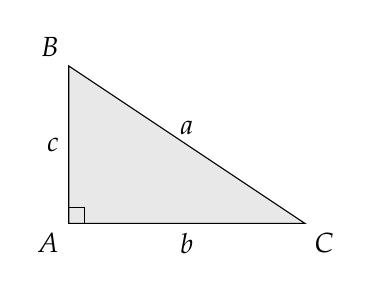
\begin{tikzpicture}

	\coordinate (A) at (0,0);
	\coordinate (B) at (0,2);
	\coordinate (C) at (3,0);

	\filldraw[fill=Gainsboro!65, draw=black] (A) -- (B) -- (C) -- cycle;
	\draw ($ (A)+(0.2,0) $) -- ++(0,0.2) -- ++(-0.2,0);

	\draw[above left] (B) node {$B$};
	\draw[below left] (A) node {$A$};
	\draw[below right] (C) node {$C$};

	\only<2->{
		\node[above] at ($ (B)!0.5!(C) $) {$a$};
		\node[left] at ($ (A)!0.5!(B) $) {$c$};
		\node[below] at ($ (A)!0.5!(C) $) {$b$};
	}

\end{tikzpicture}
		}
    \pars
		\uncover<2->{			
			Label the three sides $a$, $b$ and $c$. The side $a$, opposite the right angle, is called the {\bf hypotenuse}. \parm
		}
		\uncover<3>{ If we know the lengths of any two sides, we can calculate the length of the third side using the {\bfseries Pythagorean Theorem}:
			\par
			% centered minipage with text raggedright
			%cmini[width]{content}
			\cmini[0.5]{
				\begin{redbox}
					\[ a^2 = b^2 + c^2 \]
				\end{redbox}
			}
		} % end \only<2>
	} % end \cmini[0.8]
\end{frame}

%%%%%%%%%%%%%%%%%%%%%%%%%%%%%%%%%%%%%%%%%%%%%%%%%%%%%%%%%%%%%%%%

\begin{frame}{Right Triangle Exercises (1)}
	\centering
	% \tcb[colback=yellow]		
	\tcb		
		{			
			
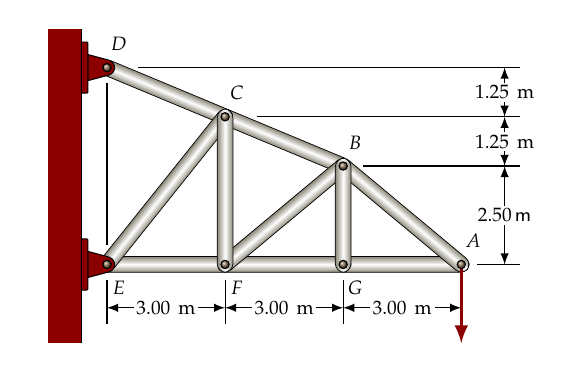
\begin{tikzpicture}



	\def\offset{0.2}
	
	\coordinate (E) at (0,0);
	\coordinate (F) at (1.5,0);
	\coordinate (G) at (3,0);
	\coordinate (A) at (4.5,0);
	\coordinate (B) at (3,1.25);
	\coordinate (C) at (1.5,1.875);
	\coordinate (D) at (0,2.5);
	\coordinate (Right) at ($ (A)+(0.75,0)$);
	\coordinate (Bottom) at ($ (A)+(0,-0.75)$);

	\fill[statsMaroon] ($(D)+(-0.325,0.5)$) rectangle ($(E)+(-.75,-1)$);
	\draw ($(D)+(-0.325,0.5)$) -- ($(E)+(-0.325,-1)$);


	\gettikzxy{(A)}{\ax}{\ay}
	\gettikzxy{(B)}{\bx}{\by}
	\gettikzxy{(C)}{\cx}{\cy}
	\gettikzxy{(D)}{\ddx}{\ddy}
	\gettikzxy{(E)}{\ex}{\ey}
	\gettikzxy{(F)}{\fx}{\fy}
	\gettikzxy{(G)}{\gx}{\gy}
	\gettikzxy{(Right)}{\rx}{\ry}
	\gettikzxy{(Bottom)}{\bbx}{\bby}

	\draw ($ (A)+(\offset,0)$) -- (\rx,\ay);
	\draw ($ (B)+(1.25*\offset,0)$) -- (\rx,\by);
	\draw ($ (C)+(2*\offset,0)$) -- (\rx,\cy);
	\draw ($ (D)+(2*\offset,0)$) -- (\rx,\ddy);
	\draw ($ (D)+(0, -\offset)$) -- (\ex,\ey+1.25*\offset cm);
	\draw ($ (E)+(0, -\offset)$) -- (\ex,\bby);
	\draw ($ (F)+(0, -\offset)$) -- (\fx,\bby);
	\draw ($ (G)+(0, -\offset)$) -- (\gx,\bby);
	\draw ($ (A)+(0, -\offset)$) -- (\ax,\bby);

	\small
	\draw[latex-latex] (\ex,\bby+\offset cm) -- node[fill=white, inner sep=0.35mm] {\scriptsize $3.00\,$ m}(\fx,\bby+\offset cm);
	\draw[latex-latex] (\fx,\bby+\offset cm) -- node[fill=white, inner sep=0.35mm] {\scriptsize $3.00\,$ m}(\gx,\bby+\offset cm);
	\draw[latex-latex] (\gx,\bby+\offset cm) -- node[fill=white, inner sep=0.35mm] {\scriptsize $3.00\,$ m}(\ax,\bby+\offset cm);
	\draw[latex-latex] (\rx-\offset cm,\ay) -- node[fill=white, inner sep=0.35mm] {\scriptsize $2.50\,\mathsf{ m}$}(\rx-\offset cm,\by);
	\draw[latex-latex] (\rx-\offset cm,\by) -- node[fill=white, inner sep=0.35mm] {\scriptsize $1.25\,$ m}(\rx-\offset cm,\cy);
	\draw[latex-latex] (\rx-\offset cm,\cy) -- node[fill=white, inner sep=0.35mm] {\scriptsize $1.25\,$ m}(\rx-\offset cm,\ddy);
	\normalsize

	% \pgfoonew \BC=new rr(B,C,Burlywood1,black, 0.2)
	% \pgfoonew \CD=new rr(C,D,Burlywood1,black, 0.2)
	% \pgfoonew \EF=new rr(E,F,Burlywood1,black, 0.2)
	% \pgfoonew \FG=new rr(G,F,Burlywood1,black, 0.2)
	% \pgfoonew \AG=new rr(A,G,Burlywood1,black, 0.2)
	% \pgfoonew \AB=new rr(A,B,Burlywood1,black, 0.2)
	% \pgfoonew \CE=new rr(C,E,Burlywood1,black, 0.2)
	% \pgfoonew \BF=new rr(B,F,Burlywood1,black, 0.2)
	% \pgfoonew \CF=new rr(C,F,Burlywood1,black, 0.2)
	% \pgfoonew \BG=new rr(B,G,Burlywood1,black, 0.2)

	 
	 \Member{B}{C}{Cornsilk4}{white}{black}{0.2}{1.125}{0.25}
	 \Member{C}{D}{Cornsilk4}{white}{black}{0.2}{1.125}{0.25}
	 \Member{A}{G}{Cornsilk4}{white}{black}{0.2}{1.125}{0.25}
	 \Member{A}{B}{Cornsilk4}{white}{black}{0.2}{1.125}{0.25}
	 \Member{F}{G}{Cornsilk4}{white}{black}{0.2}{1.125}{0.25}
	 \Member{F}{E}{Cornsilk4}{white}{black}{0.2}{1.125}{0.25}
	 \Member{B}{F}{Cornsilk4}{white}{black}{0.2}{1.125}{0.25}
	 \Member{B}{G}{Cornsilk4}{white}{black}{0.2}{1.125}{0.25}
	 \Member{C}{E}{Cornsilk4}{white}{black}{0.2}{1.125}{0.25}
	 \Member{C}{F}{Cornsilk4}{white}{black}{0.2}{1.125}{0.25}

	\PC[-90]{D}{statsMaroon}{black}{0.325}{0.125}
	\PC[-90]{E}{statsMaroon}{black}{0.325}{0.125}

	\draw[very thick, statsMaroon, -latex] (A) -- +(0,-1);

	\shadedraw[ball color=Burlywood4] (A) circle (1.5pt) node[xshift=1.5mm, yshift=3mm] {\scriptsize $A$};
	\shadedraw[ball color=Burlywood4] (B) circle (1.5pt) node[xshift=1.5mm, yshift=3mm] {\scriptsize $B$};
	\shadedraw[ball color=Burlywood4] (C) circle (1.5pt) node[xshift=1.5mm, yshift=3mm] {\scriptsize $C$};
	\shadedraw[ball color=Burlywood4] (D) circle (1.5pt) node[xshift=1.5mm, yshift=3mm] {\scriptsize $D$};
	\shadedraw[ball color=Burlywood4] (E) circle (1.5pt) node[xshift=1.5mm, yshift=-3mm] {\scriptsize $E$};
	\shadedraw[ball color=Burlywood4] (F) circle (1.5pt) node[xshift=1.5mm, yshift=-3mm] {\scriptsize $F$};
	\shadedraw[ball color=Burlywood4] (G) circle (1.5pt) node[xshift=1.5mm, yshift=-3mm] {\scriptsize $G$};
\pgfresetboundingbox
\draw[white] ($ (D)+ (-1,0.5) $) rectangle ($ (A)+(1,-1) $);

\end{tikzpicture}

		}
	\cmini[0.65]{
		\begin{enumerate}
			\setcounter{enumi}{\themyexercisecounter}
			\item  Use the Pythagorean Theorem to determine the lengths of $CE$ and $CB$
			\setcounter{myexercisecounter}{\theenumi}
		\end{enumerate}
	}

	\vfill

	% answers, gray, centered, upside down	
	% \footnotesize
	% \textcolor{gray}{
	% 	\rotatebox[origin=c]{180}{
	% 		($CE=4.80\text{ m},\, CD=3.25\text{ m} $ )
	% 	}
	% }

\end{frame}
%%%%%%%%%%%%%%%%%%%%%%%%%%%%%%%%%%%%%%%%%%%%%%%%%%%%%%%%%%%%%%%%
\begin{frame}{Significant Digits}
	\cmini[0.9]{
    \begin{redbox}
      \begin{itemize}
        \item Significant {\bf  digits} and significant {\bf figures} are the same thing.
        \parb\pause
        \item Significant digits are a measure of the {\bf accuracy} of a number.
        \parb\pause
        {\small It is \textcolor{structure}{\bf extremely important} to recognize that we can get 	no more accuracy out of a calculation than we put in. If the inputs to a
				problem have three significant digits, we cannot expect any higher
				accuracy than three significant digits in our result --- even if the
				calculator does give ten digits.}
      \end{itemize}
    \end{redbox}
	}
\end{frame}

%%%%%%%%%%%%%%%%%%%%%%%%%%%%%%%%%%%%%%%%%%%%%%%%%%%%%%%%%%%%%%%%
\begin{frame}{Significant Digits}

	\cmini[0.8]{
    \begin{titledbox}{Non-zero digits}
      Non-zero digits {\bf are} significant:
      \begin{itemize}
			      	\item $1234$ has $\color{statsMaroon}{4}$ significant digits.			      	
			      	\item $12.34$ has $\color{statsMaroon}{4}$ significant digits.
			      \end{itemize}
    \end{titledbox}
    \pause\parb
    \begin{titledbox}{Zeros between non-zero digits are significant}
      \begin{itemize}
			      	\item $12034$ has $\color{statsMaroon}{5}$ significant digits.			      	
			      	\item $12.0034$ has $\color{statsMaroon}{6}$ significant digits.
			      \end{itemize}
    \end{titledbox}   
	}

\end{frame}
%%%%%%%%%%%%%%%%%%%%%%%%%%%%%%%%%%%%%%%%%%%%%%%%%%%%%%%%%%%%%%%%
\begin{frame}{Significant Digits}
 
	\cmini[0.8]{
    \begin{titledbox}{Leading zeros are {\bf not} significant}
      \begin{itemize}			      	
        \item $0.1234$ has $\color{statsMaroon}{4}$ significant digits.
        \item $0.0001234$ has $\color{statsMaroon}{4}$ significant digits.
      \end{itemize}          
    \end{titledbox}
    \pause\pars
    \begin{titledbox}{Trailing zeros (after a decimal point) {\bf are} significant}
      \begin{itemize}			      	
        \item $1234.0$ has $\color{statsMaroon}{5}$ significant digits.
        \item $1.23400$ has $\color{statsMaroon}{6}$ significant digits.
      \end{itemize}          
    \end{titledbox}			 
	}

\end{frame}
%%%%%%%%%%%%%%%%%%%%%%%%%%%%%%%%%%%%%%%%%%%%%%%%%%%%%%%%%%%%%%%%
\begin{frame}{Significant Digits}
 
	\cmini[0.8]{
           
   
    \begin{titledbox}{Trailing zeros (on whole numbers, i.e.\! integers) are more {\bf complicated}}
      \begin{itemize}			      	
        \item $12300$ can have $\color{statsMaroon}{3}$, $\color{statsMaroon}{4}$ or $\color{statsMaroon}{5}$ significant digits!\parm\pause
        \begin{itemize}
					\item Consider $12.3\,$m. This value has $\color{statsMaroon}{3}$ significant digits. It is equal to $12300\,$mm, so in this case the $12300$ also has $\color{statsMaroon}{3}$ significant digits.\parm\pause
					\item Now consider $12.30\,$m. This value has $\color{statsMaroon}{4}$ significant digits. But it is still equal to $12300\,$mm, so in this case the $12300$ has $\color{statsMaroon}{4}$ significant digits.\parm\pause
					\item What if $12300\,$mm refers to $12.300\,$m? Then it has $\color{statsMaroon}{5}$ significant digits.\pause
				\end{itemize}
				\item Usually, the trailing zeros are placeholders for the magnitude of a value and we don't need to worry unduly.\pause
				\item If we want to emphasize that $12300$ has $\color{statsMaroon}{4}$ significant digits, we can write $1.230\x\left(10^3\right)$.
      \end{itemize}          
    \end{titledbox}
	}

\end{frame}

% %%%%%%%%%%%%%%%%%%%%%%%%%%%%%%%%%%%%%%%%%%%%%%%%%%%%%%%%%%%%%%%%%%%%%%%%%%%%%%%%

\begin{frame}{Calculations for Exercises}
	\cmini[0.8]{
		\begin{itemize}
			\item In practice, it is often difficult to measure objects more accurately than to three significant digits so {\bfseries input values for exercises are generally given to $\color{statsMaroon}{3}$ significant digits}. 
			% ({\small Or sometimes $\color{statsMaroon}{4}$ significant digits when the leading significant digit is a $\color{statsMaroon}{1}$})
      \parm\pause
			\item We cannot expect to get more accuracy in our result at the end of a calculation than from our given input values at the beginning of the calculation so {\bfseries solutions should be correct to $\color{statsMaroon}{3}$ significant digits, not more than the accuracy of the calculation inputs! }\parm\pause
			\item Intermediate calculations will accumulate rounding errors quickly if we use only three significant digits and these can affect the final result. {\bfseries For intermediate calculations, use $\color{statsMaroon}{5}$ or more significant digits.}\parm
			{\small (When I write solutions down, I use $5$ significant digits for intermediate calculations. You may use more if it is more convenient for you, e.g., if you are storing intermediate results in your calculator.)}
		\end{itemize}
	}

\end{frame}
% %%%%%%%%%%%%%%%%%%%%%%%%%%%%%%%%%%%%%%%%%%%%%%%%%%%%%%%%%%%%%%%%%%%%%%%%%%%%%%%%

\begin{frame}{Significant Digits and Rounding}
	\cmini[0.8]{
		\begin{itemize}
			\item When using five significant digits for intermediate calculations, it is necessary to convert back to three significant digits when providing the final answer to an exercise. Then, {\bf rounding} is often involved:
      \parm\pause
			\begin{itemize}
				\item $2.3456$ becomes $2.35$ because the first non-significant digit (the $5$ in
				this case) is $\ge 5$ and so the $4$ rounds up.\pars\pause
				\item $2.3446$ becomes $2.34$ because the first non-significant digit (the $4$ in
				this case) is $< 5$ and the last significant digit, $4$, remains unchanged.\pause
			\end{itemize}
			\item When the first discarded digit is a $5$ (or higher), round up the digit
			before the $5$ (or higher)\parm\pause
			\item There are various rules (such as the odd-even rule) which take a
			more complicated approach to rounding $5$ but, for our purposes, $\bm 5$ {\bf rounds up}!
		\end{itemize}
	}
\end{frame}

%%%%%%%%%%%%%%%%%%%%%%%%%%%%%%%%%%%%%%%%%%%%%%%%%%%%%%%%%%%%%%%%%%%%%%%%%%%%%%%%

\begin{frame}{More About Right Triangle}
	
	\cmini[0.8]{
		The sine, cosine and tangent trigonometrical functions relate an acute angle ($\theta$, in this example) in a right triangle to two of the sides of the triangle.
		\parm
		\begin{center}
			\tcb		
				{			
					% !TEX root = ../../Presentations/01MathReview/01STCS200MathReview.tex

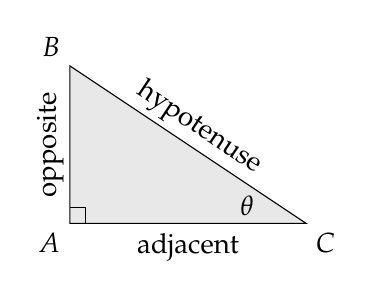
\begin{tikzpicture}

	\coordinate (A) at (0,0);
	\coordinate (B) at (0,2);
	\coordinate (C) at (3,0);

	\filldraw[fill=Gainsboro!65, draw=black] (A) -- (B) -- (C) -- cycle;
	\draw ($ (A)+(0.2,0) $) -- ++(0,0.2) -- ++(-0.2,0);

	\draw[above left] (B) node {$B$};
	\draw[below left] (A) node {$A$};
	\draw[below right] (C) node {$C$};

	
		\path (B) -- (C) node[midway, sloped, yshift=0.25cm] {hypotenuse};
		\path (A) -- (B) node[midway, sloped, yshift=0.25cm] {opposite};
		\node[below] at ($ (A)!0.5!(C) $) {adjacent};
		\node at ($ (C)+(-0.75,0.225) $) {$\theta$};


\end{tikzpicture}
				}
		\end{center}
		\pause
	} % end cmini

	\begin{statsbox}[top=0mm]{Right Triangle Trigonometry Formul\ae}
		\centering
		$$		
		\sin\theta = \frac{{\bm o}\text{\textcolor{gray}{pposite}}}{{\bm h}\text{\textcolor{gray}{ypotenuse}}}, \quad
		\cos\theta = \frac{{\bm a}\text{\textcolor{gray}{djacent}}}{{\bm h}\text{\textcolor{gray}{ypotenuse}}},
		\quad
		\tan\theta = \frac{{\bm o}\text{\textcolor{gray}{pposite}}}{{\bm a}\text{\textcolor{gray}{djacent}}}
		$$
  \end{statsbox}
	\centering
	Remember: {\bfseries SOHCAHTOA}

	

\end{frame}
%%%%%%%%%%%%%%%%%%%%%%%%%%%%%%%%%%%%%%%%%%%%%%%%%%%%%%%%%%%%%%%%%%%%%%%%%%%%%%%%

\begin{frame}{Right Triangle Exercises (2)}
	%cmini[width]{content}
	\cmini[0.85]{
		\centering
		\tcb[right=2mm]{
			
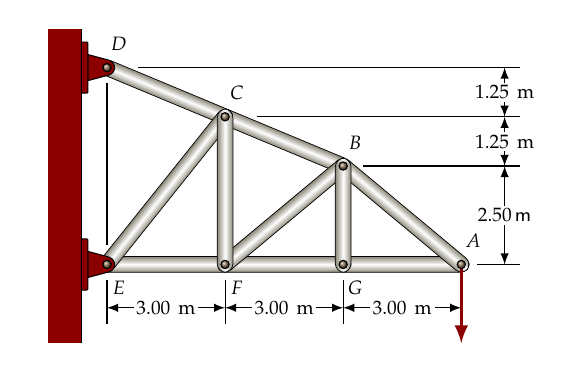
\begin{tikzpicture}



	\def\offset{0.2}
	
	\coordinate (E) at (0,0);
	\coordinate (F) at (1.5,0);
	\coordinate (G) at (3,0);
	\coordinate (A) at (4.5,0);
	\coordinate (B) at (3,1.25);
	\coordinate (C) at (1.5,1.875);
	\coordinate (D) at (0,2.5);
	\coordinate (Right) at ($ (A)+(0.75,0)$);
	\coordinate (Bottom) at ($ (A)+(0,-0.75)$);

	\fill[statsMaroon] ($(D)+(-0.325,0.5)$) rectangle ($(E)+(-.75,-1)$);
	\draw ($(D)+(-0.325,0.5)$) -- ($(E)+(-0.325,-1)$);


	\gettikzxy{(A)}{\ax}{\ay}
	\gettikzxy{(B)}{\bx}{\by}
	\gettikzxy{(C)}{\cx}{\cy}
	\gettikzxy{(D)}{\ddx}{\ddy}
	\gettikzxy{(E)}{\ex}{\ey}
	\gettikzxy{(F)}{\fx}{\fy}
	\gettikzxy{(G)}{\gx}{\gy}
	\gettikzxy{(Right)}{\rx}{\ry}
	\gettikzxy{(Bottom)}{\bbx}{\bby}

	\draw ($ (A)+(\offset,0)$) -- (\rx,\ay);
	\draw ($ (B)+(1.25*\offset,0)$) -- (\rx,\by);
	\draw ($ (C)+(2*\offset,0)$) -- (\rx,\cy);
	\draw ($ (D)+(2*\offset,0)$) -- (\rx,\ddy);
	\draw ($ (D)+(0, -\offset)$) -- (\ex,\ey+1.25*\offset cm);
	\draw ($ (E)+(0, -\offset)$) -- (\ex,\bby);
	\draw ($ (F)+(0, -\offset)$) -- (\fx,\bby);
	\draw ($ (G)+(0, -\offset)$) -- (\gx,\bby);
	\draw ($ (A)+(0, -\offset)$) -- (\ax,\bby);

	\small
	\draw[latex-latex] (\ex,\bby+\offset cm) -- node[fill=white, inner sep=0.35mm] {\scriptsize $3.00\,$ m}(\fx,\bby+\offset cm);
	\draw[latex-latex] (\fx,\bby+\offset cm) -- node[fill=white, inner sep=0.35mm] {\scriptsize $3.00\,$ m}(\gx,\bby+\offset cm);
	\draw[latex-latex] (\gx,\bby+\offset cm) -- node[fill=white, inner sep=0.35mm] {\scriptsize $3.00\,$ m}(\ax,\bby+\offset cm);
	\draw[latex-latex] (\rx-\offset cm,\ay) -- node[fill=white, inner sep=0.35mm] {\scriptsize $2.50\,\mathsf{ m}$}(\rx-\offset cm,\by);
	\draw[latex-latex] (\rx-\offset cm,\by) -- node[fill=white, inner sep=0.35mm] {\scriptsize $1.25\,$ m}(\rx-\offset cm,\cy);
	\draw[latex-latex] (\rx-\offset cm,\cy) -- node[fill=white, inner sep=0.35mm] {\scriptsize $1.25\,$ m}(\rx-\offset cm,\ddy);
	\normalsize

	% \pgfoonew \BC=new rr(B,C,Burlywood1,black, 0.2)
	% \pgfoonew \CD=new rr(C,D,Burlywood1,black, 0.2)
	% \pgfoonew \EF=new rr(E,F,Burlywood1,black, 0.2)
	% \pgfoonew \FG=new rr(G,F,Burlywood1,black, 0.2)
	% \pgfoonew \AG=new rr(A,G,Burlywood1,black, 0.2)
	% \pgfoonew \AB=new rr(A,B,Burlywood1,black, 0.2)
	% \pgfoonew \CE=new rr(C,E,Burlywood1,black, 0.2)
	% \pgfoonew \BF=new rr(B,F,Burlywood1,black, 0.2)
	% \pgfoonew \CF=new rr(C,F,Burlywood1,black, 0.2)
	% \pgfoonew \BG=new rr(B,G,Burlywood1,black, 0.2)

	 
	 \Member{B}{C}{Cornsilk4}{white}{black}{0.2}{1.125}{0.25}
	 \Member{C}{D}{Cornsilk4}{white}{black}{0.2}{1.125}{0.25}
	 \Member{A}{G}{Cornsilk4}{white}{black}{0.2}{1.125}{0.25}
	 \Member{A}{B}{Cornsilk4}{white}{black}{0.2}{1.125}{0.25}
	 \Member{F}{G}{Cornsilk4}{white}{black}{0.2}{1.125}{0.25}
	 \Member{F}{E}{Cornsilk4}{white}{black}{0.2}{1.125}{0.25}
	 \Member{B}{F}{Cornsilk4}{white}{black}{0.2}{1.125}{0.25}
	 \Member{B}{G}{Cornsilk4}{white}{black}{0.2}{1.125}{0.25}
	 \Member{C}{E}{Cornsilk4}{white}{black}{0.2}{1.125}{0.25}
	 \Member{C}{F}{Cornsilk4}{white}{black}{0.2}{1.125}{0.25}

	\PC[-90]{D}{statsMaroon}{black}{0.325}{0.125}
	\PC[-90]{E}{statsMaroon}{black}{0.325}{0.125}

	\draw[very thick, statsMaroon, -latex] (A) -- +(0,-1);

	\shadedraw[ball color=Burlywood4] (A) circle (1.5pt) node[xshift=1.5mm, yshift=3mm] {\scriptsize $A$};
	\shadedraw[ball color=Burlywood4] (B) circle (1.5pt) node[xshift=1.5mm, yshift=3mm] {\scriptsize $B$};
	\shadedraw[ball color=Burlywood4] (C) circle (1.5pt) node[xshift=1.5mm, yshift=3mm] {\scriptsize $C$};
	\shadedraw[ball color=Burlywood4] (D) circle (1.5pt) node[xshift=1.5mm, yshift=3mm] {\scriptsize $D$};
	\shadedraw[ball color=Burlywood4] (E) circle (1.5pt) node[xshift=1.5mm, yshift=-3mm] {\scriptsize $E$};
	\shadedraw[ball color=Burlywood4] (F) circle (1.5pt) node[xshift=1.5mm, yshift=-3mm] {\scriptsize $F$};
	\shadedraw[ball color=Burlywood4] (G) circle (1.5pt) node[xshift=1.5mm, yshift=-3mm] {\scriptsize $G$};
\pgfresetboundingbox
\draw[white] ($ (D)+ (-1,0.5) $) rectangle ($ (A)+(1,-1) $);

\end{tikzpicture}

		}
		\par
		\begin{enumerate}
			\setcounter{enumi}{\themyexercisecounter}
			\item Use the {\bfseries tangent} function to calculate $\angle CEF$.
			      % {\footnotesize
			      % 	\textcolor{gray}{
			      % 		\rotatebox[origin=c, y=2.5pt]{180}{
			      % 			( $51.3^\circ$)
			      % 		}
			      % 	}
			      % }			      

			\item From $\angle CEF$ just found ({\bfseries use the intermediate, 5 or more significant digit, form!}) and the {\bfseries sine} rule to verify the length of $CE$ found earlier.


			\item Use the {\bfseries cosine} function and the length of $CB$ found earlier to calculate the angle between $BC$ and the horizontal. 
			
			% {\footnotesize\textcolor{gray}{\rotatebox[origin=c, y=2.5pt]{180}{($22.6^\circ$ )}}}

			\item Use the {\bfseries tangent} function to verify the previous result.
			      \setcounter{myexercisecounter}{\theenumi}
		\end{enumerate}
	}
\end{frame}
%%%%%%%%%%%%%%%%%%%%%%%%%%%%%%%%%%%%%%%%%%%%%%%%%%%%%%%%%%%%%%%%%%%%%%%%%%%%%%%%
\begin{frame}{Triangles - Sine Rule}
	% centered minipage with text raggedright
	%cmini[width]{content}
	\cmini[0.9]{
		\centering
		Not all triangles contain a right angle. To solve for these triangles (finding the lengths of the side and the triangle angles), we have to employ some different tools: 	 the {\bfseries sine rule} and (later) the {\bfseries cosine rule}
		\parm
		\centering
		\tcb{% !TEX root = ../../Beamer/statikz/statikz.tex


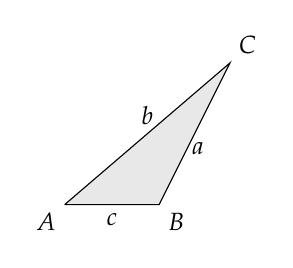
\begin{tikzpicture}[scale=0.6]

	\coordinate (A) at (0,0);
	\coordinate (B) at (2,0);
	\coordinate (C) at (3.5,3);

	\small
	\filldraw[fill=Gainsboro!65, draw=black] (A) -- node[below] {$c$}(B) --  node[below] { \;$a$}(C) --  node[above] {$b$} (A);

	\draw[below right] (B) node {$B$};
	\draw[below left] (A) node {$A$};
	\draw[above right] (C) node {$C$};
	
\end{tikzpicture}
}
	}
	% centered minipage with text raggedright
	%cmini[width]{content}
	\cmini[0.9]{
		\mini[0.45]{
			\centering
			\begin{statsbox}[top=0mm]{Sine Rule}
				\[ \frac{\sin A}{a} = \frac{\sin B}{b}=\frac{\sin C}{c} \]
			\end{statsbox}
		}
		or
		\mini[0.45]{
			\begin{statsbox}[top=0mm]{Sine Rule}
				\[ \frac{a}{\sin A} = \frac{b}{\sin B}=\frac{c}{\sin C} \]
			\end{statsbox}
		}
	}
\end{frame}

%%%%%%%%%%%%%%%%%%%%%%%%%%%%%%%%%%%%%%%%%%%%%%%%%%%%%%%%%%%%%%%%%%%%%%%%%%%%%%%%

\begin{frame}{Triangles - Sine Rule Exercises}

	\mini[0.6]{
		\begin{enumerate}
			\setcounter{enumi}{\themyexercisecounter}
			\item Using the sine rule, find $\angle ACB$. 
			% {\footnotesize\textcolor{gray}{\rotatebox[origin=c, y=2.5pt]{180}{($95.8^\circ$)}}}
					      
			\item Using the sine rule, find $\angle ABC$. 
			% {\footnotesize\textcolor{gray}{\rotatebox[origin=c, y=2.5pt]{180}{($28.2^\circ$)}}}
			\item Sum the interior angles of the triangle. 
			      \setcounter{myexercisecounter}{\theenumi}
		\end{enumerate}
	}
	\mini[0.35]{
		\centering
		\tcb{% !TEX root = ../../Beamer/statikz/statikz.tex


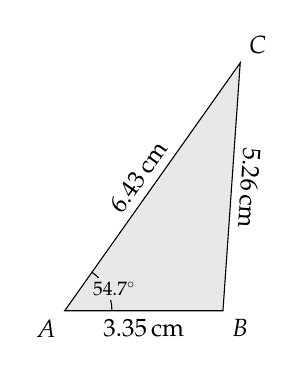
\begin{tikzpicture}[scale=0.6]

	\coordinate (A) at (0,0);
	\coordinate (B) at ($ (A)+(3.35, 0)$);
	\coordinate (C) at ($ (A)+(54.7:6.43)$);
	
  

	\small
	\filldraw[fill=Gainsboro!65, draw=black] (A) -- (B) --  (C) --  cycle;
  
	\path (A) -- (C) node[midway, sloped, above] {$6.43\,$cm};
	\path (C) -- (B) node[midway, sloped, above, rotate=180] {$5.26\,$cm};
	\path (A) -- (B) node[midway, sloped, below] {$3.35\,$cm};
	\draw[below right] (B) node {$B$};
	\draw[below left] (A) node {$A$};
	\draw[above right] (C) node {$C$};

	\draw ($ (A)+(54.7:1) $) arc (54.7:0:1)node[midway, fill=Gainsboro!65, inner sep=0.5mm,xshift=1mm] {\scriptsize $ 54.7\deg $};
  

	% \node[xshift=-0.5cm, yshift=0.15cm] at (C) {$\theta $};



\end{tikzpicture}
}
	}
\end{frame}

%%%%%%%%%%%%%%%%%%%%%%%%%%%%%%%%%%%%%%%%%%%%%%%%%%%%%%%%%%%%%%%%%%%%%%%%%%%%%%%%

%%%%%%%%%%%%%%%%%%%%%%%%%%%%%%%%%%%%%%%%%%%%%%%%%%%%%%%%%%%%%%%%%%%%%%%%%%%%%%%%

\begin{frame}{Trig Identities}
	\setlength{\tabcolsep}{1mm}
	% centered minipage with text raggedright
	%cmini[width]{content}
	\cmini[0.8]{
		\centering
		A couple of trig identities that will come in useful:
		\tcbtl[left=5mm, right=5mm]{Identities}{%
		% align* doesn't seem to work in tcbox but aligned does when in math mode
		$\begin{aligned}
			\sin\left(180\deg-\theta\right) &=\sin\theta\\
			\cos\left(-\theta\right) &= \cos\theta
		\end{aligned}$
		}
		\parb
		\begin{statsbox}[left=5mm, right=5mm]{Note:}
			\centering
			\begin{tabular}{rcccl}
				$\sin(140\deg)$ &=& $\sin(40\deg)$ &=& $0.64279$\\
				$\cos(42\deg)$ &=& $\cos(-42\deg)$ &=& $0.74314$\\
			\end{tabular}
			\parb
			Thus, we have to be careful when using inverse trigonometric functions:
			\parb
			\begin{tabular}{rcccl}
				$\sin^{-1}(0.64279)$ &=& $40\deg$ &or& $140\deg$\\
				$\cos^{-1}0.74314)$ &=& $-42\deg$ &or& $42\deg$\\
			\end{tabular}
		\end{statsbox}
	}

	
	
\end{frame}
%%%%%%%%%%%%%%%%%%%%%%%%%%%%%%%%%%%%%%%%%%%%%%%%%%%%%%%%%%%%%%%%%%%%%%%%%%%%%%%%
\begin{frame}{Triangles - Cosine Rule}
	% centered minipage with text raggedright
	%cmini[width]{content}
	\cmini[0.8]{
		\centering
		\tcb{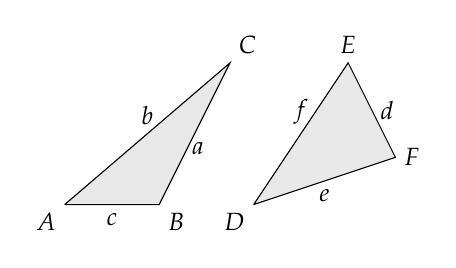
\begin{tikzpicture}[scale=0.6]

	\coordinate (A) at (0,0);
	\coordinate (B) at (2,0);
	\coordinate (C) at (3.5,3);
  \coordinate (D) at (4,0);
	\coordinate (E) at (6,3);
	\coordinate (F) at (7,1);

	\small
	\filldraw[fill=Gainsboro!65, draw=black] (A) -- node[below] {$c$}(B) --  node[below] { \;$a$}(C) --  node[above] {$b$} (A);
  \filldraw[fill=Gainsboro!65, draw=black] (D) -- node[above] {$f$}(E) --  node[right] {$d$}(F) --  node[below] {$e$} (D);

	\draw[below right] (B) node {$B$};
	\draw[below left] (A) node {$A$};
	\draw[above right] (C) node {$C$};
  \draw[below left] (D) node {$D$};
	\draw[above] (E) node {$E$};
	\draw[right] (F) node {$F$};
\end{tikzpicture}
}
	}
	% centered minipage with text raggedright
	%cmini[width]{content}
	\cmini[0.6]{
		\begin{statsbox}[top=0 mm]{Cosine Rule}
			\begin{align*}
				a^2 & = b^2 + c^2 -2bc\cos A \\
				b^2 & = a^2 + c^2 -2ac\cos B \\
				c^2 & = a^2 + b^2 -2ab\cos C 
			\end{align*}
		\end{statsbox}
		\parm
		The cosine rule is useful when you have all the sides of a triangle and want to find the angles.

	}
\end{frame}

%%%%%%%%%%%%%%%%%%%%%%%%%%%%%%%%%%%%%%%%%%%%%%%%%%%%%%%%%%%%%%%%%%%%%%%%%%%%%%%%

\begin{frame}{Triangles - Cosine Rule Exercises}

	\mini[0.5]{
		\begin{enumerate}
			\setcounter{enumi}{\themyexercisecounter}
			\item Determine $\angle ABC$, using the value for $AB$ found earlier
			\item Compare the value for $\angle ABC$ with the value calculated earlier. \lb Is it the same? It should be!
			      \setcounter{myexercisecounter}{\theenumi}
		\end{enumerate}
	}
	\mini[0.4]{
		\centering
		\tcb{% !TEX root = ../../Beamer/statikz/statikz.tex


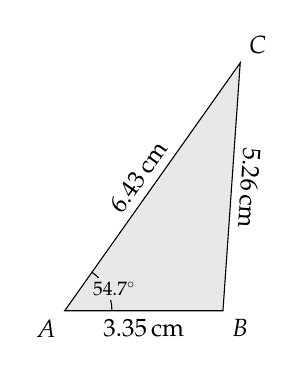
\begin{tikzpicture}[scale=0.6]

	\coordinate (A) at (0,0);
	\coordinate (B) at ($ (A)+(3.35, 0)$);
	\coordinate (C) at ($ (A)+(54.7:6.43)$);
	
  

	\small
	\filldraw[fill=Gainsboro!65, draw=black] (A) -- (B) --  (C) --  cycle;
  
	\path (A) -- (C) node[midway, sloped, above] {$6.43\,$cm};
	\path (C) -- (B) node[midway, sloped, above, rotate=180] {$5.26\,$cm};
	\path (A) -- (B) node[midway, sloped, below] {$3.35\,$cm};
	\draw[below right] (B) node {$B$};
	\draw[below left] (A) node {$A$};
	\draw[above right] (C) node {$C$};

	\draw ($ (A)+(54.7:1) $) arc (54.7:0:1)node[midway, fill=Gainsboro!65, inner sep=0.5mm,xshift=1mm] {\scriptsize $ 54.7\deg $};
  

	% \node[xshift=-0.5cm, yshift=0.15cm] at (C) {$\theta $};



\end{tikzpicture}
}
	}
\end{frame}

%%%%%%%%%%%%%%%%%%%%%%%%%%%%%%%%%%%%%%%%%%%%%%%%%%%%%%%%%%%%%%%%%%%%%%%%%%%%%%%%

\begin{frame}{Similar Triangles}
	\begin{center}
		\tcb{% !TEX root = ../../Beamer/statikz/statikz.tex


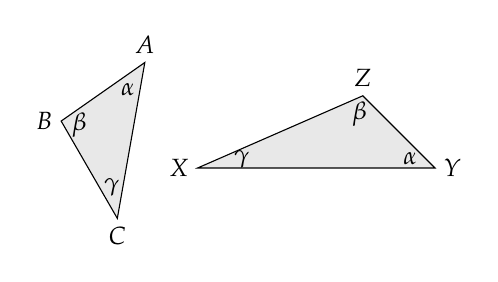
\begin{tikzpicture}[scale=0.67]

	\coordinate (A) at (0,0);
	\coordinate (B) at ($(A)+(215:1.936)  $);
	\coordinate (C) at ($ (B)+(-60:2.129) $);
  \coordinate (X) at (1,-2);
	\coordinate (Y) at ($ (X)+(0:4.5) $);
	\coordinate (Z) at ($ (Y)+(135:1.936) $);

	\small
	\filldraw[fill=Gainsboro!65, draw=black] (A) -- (B) -- (C) -- cycle;
  \filldraw[fill=Gainsboro!65, draw=black] (X) -- (Y) -- (Z) -- cycle;

	\draw[left] (B) node {$B$};
	\draw[above] (A) node {$A$};
	\draw[below] (C) node {$C$};
  \draw[left] (X) node {$X$};
	\draw[right] (Y) node {$Y$};
	\draw[above] (Z) node {$Z$};

	\node at ($(C)+(100:0.6)$) {$\gamma $};
	\node at ($(B)+(-12.5:0.35)$) {$\beta $};
	\node at ($(A)+(-122.5:0.6)$) {$\alpha $};
	\node at ($(X)+(11:0.85)$) {$\gamma $};
	\node at ($(Z)+(-100:0.35)$) {$\beta $};
	\node at ($(Y)+(160:0.5)$) {$\alpha $};



\end{tikzpicture}
}
	\end{center}
	% centered minipage with text raggedright
	%cmini[width]{content}
	\cmini[0.7]{
		\centering
		If triangles $ABC$ and $XYZ$ have the same angles, they are said to be {\bfseries similar triangles}.
		\parm\pause
		The ratios of the lengths of corresponding sides of similar triangles are equal:
		\parm
		\centering
		\tcb[left=5mm,right=5mm]{
			$ \frac{AB}{XY} = \frac{BC}{XZ} = \frac{AC}{YZ} $
		}
	}
\end{frame}
%%%%%%%%%%%%%%%%%%%%%%%%%%%%%%%%%%%%%%%%%%%%%%%%%%%%%%%%%%%%%%%%%%%%%%%%%%%%%%%%

\begin{frame}{Similar Triangles - Exercises}
	\mini[0.4]{
		\raggedright
		\normalsize
		$ABCD$ is a rigid (i.e., it does not deform) plate, pinned at $C$. \parm
		
		\uncover<2->{
			When horizontal force $P$ is applied at $A$, $ABCD$ rotates about $C$ and $A$ deflects $2.45\,$mm horizontally rightwards. \parm
			Assume that $BF$ remains horizontal and that $DE$ remains vertical.
		}
		
		
	
	
		%\uncover<2>{
			% answers, gray, centered, upside down
			% \begin{center}
			% 	\footnotesize
			% 	\textcolor{gray}{
			% 		\rotatebox[origin=c]{180}{
			% 			($\delta_{BF}=0.969\text{ mm},\,\delta_{DE}=1.319\text{ mm}$)
			% 		}
			% 	}
			% \end{center}
		%}
	}
	\hfill	
	\mini[0.55]{
		\centering	
		\tcb[top=5mm,bottom=5mm]{% !TEX root = ../../Beamer/statikz/statikz.tex

\scalebox{0.67}{
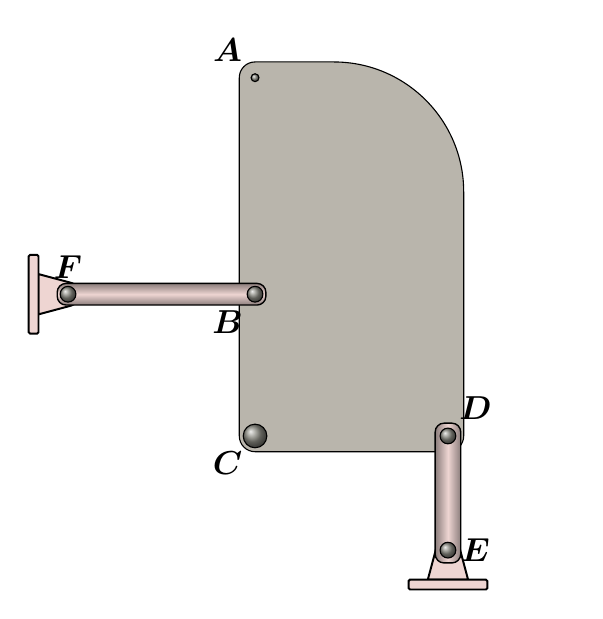
\begin{tikzpicture}[scale=1]

	\coordinate (C) at (0,0);
	\coordinate (B) at ($ (C)+(90:1.8)  $);
	\coordinate (A) at ($ (B)+(90:2.75) $);
  \coordinate (D) at ($ (C)+(0:2.45) $);
	\coordinate (E) at ($ (D)+(-90:1.45) $);
	\coordinate (F) at ($ (B)+(180:2.375) $);
	\def\delta{0.2cm}

	\gettikzxy{(A)}{\ax}{\ay}
  \gettikzxy{(B)}{\bx}{\by}
  \gettikzxy{(C)}{\cx}{\cy}
  \gettikzxy{(D)}{\ddx}{\ddy}
  \gettikzxy{(E)}{\ex}{\ey}
  \gettikzxy{(F)}{\fx}{\fy}

	\filldraw[fill=Ivory3!70!MistyRose4, draw=black] (\cx-\delta, \cy)--(\cx-\delta, \ay)arc(180:90:\delta)--+(1,0)arc(90:0:1.65)--(\ddx+\delta, \ddy)arc(0:-90:\delta)--(\cx, \cy-\delta)arc(270:180:\delta);

	\PC[270]{F}{MistyRose2}{black}{0.5}{0.25}
	\PC{E}{MistyRose2}{black}{0.5}{0.25}

	\Member{F}{B}{MistyRose4}{MistyRose2}{black}{0.275}{1.125}{0.5}
	\Member{D}{E}{MistyRose4}{MistyRose2}{black}{0.325}{1.125}{0.5}

	\small
	% \filldraw[fill=Gainsboro!65, draw=black] (A) -- (B) -- (C) -- cycle;
  % \filldraw[fill=Gainsboro!65, draw=black] (X) -- (Y) -- (Z) -- cycle;


	\large
	\shadedraw [draw=black, ball color = Ivory4] (C) circle (0.15cm) node[xshift=-0.35cm, yshift=-0.35cm] {\large $\bm C$};
	\shadedraw [draw=black, ball color = Ivory4] (B) circle (0.1cm) node[xshift=-0.35cm,yshift=-0.35cm] {$\bm B$};
	\shadedraw [draw=black, ball color = Ivory4] (A) circle (0.05cm) node[xshift=-0.35cm, yshift=0.35cm] {$\bm A$};
	\shadedraw [draw=black, ball color = Ivory4] (D) circle (0.1cm) node[yshift=0.35cm,xshift=0.35cm] {$\bm D$};
	\shadedraw [draw=black, ball color = Ivory4] (E) circle (0.1cm) node[xshift=0.35cm] {$\bm E$};
	\shadedraw [draw=black, ball color = Ivory4] (F) circle (0.1cm) node[yshift=0.35cm] {$\bm F$};
	% \node at ($(B)+(-12.5:0.35)$) {$\beta $};
	% \node at ($(A)+(-122.5:0.6)$) {$\alpha $};
	% \node at ($(X)+(11:0.85)$) {$\gamma $};
	% \node at ($(Z)+(-100:0.35)$) {$\beta $};
	% \node at ($(Y)+(160:0.5)$) {$\alpha $};



\end{tikzpicture}
}}
	}

	\cmini[0.7]{
		\parb
		% \only<1>{
		% 		\begin{enumerate}
		% 			\setcounter{enumi}{\themyexercisecounter}
		% 			\item Determine $\delta_{BF}$, the change in length of $BF$.
		% 			\item Determine $\delta_{DE}$, the change in length of $DE$.
		% 						%\setcounter{myexercisecounter}{\theenumi}
		% 		\end{enumerate}
		% 	}
			% to avoid incrementing question numbers on overlay, do not save after the first overlay.
			\uncover<3>{
				\begin{enumerate}
					\setcounter{enumi}{\themyexercisecounter}
					\item Determine $\delta_{BF}$, the change in length of $BF$.
					\item Determine $\delta_{DE}$, the change in length of $DE$.
								\setcounter{myexercisecounter}{\theenumi}
				\end{enumerate}
			}
	}
	\vspace{-0.75cm}
\end{frame}
%%%%%%%%%%%%%%%%%%%%%%%%%%%%%%%%%%%%%%%%%%%%%%%%%%%%%%%%%%%%%%%%%%%%%%%%%%%%%%%%

\begin{frame}{Right Triangles and Trigonometric Functions - Exercises}
	% \hspace{-0.5cm}
	% left-aligned minipage with text raggedright
	%mini[width]{content}
	\mini[0.55]{
		\begin{enumerate}
			\setcounter{enumi}{\themyexercisecounter}
			\item  Show that right triangles $\triangle ABC$, $\triangle ABD$ and $\triangle ACD$ all have the same angles (i.e., they are all similar).
			\item Given that $AC=100\text{ mm}$ and $AD=65\text{ mm}$, determine $\angle ACD$ and $\angle ABD$. 
			% {\footnotesize\textcolor{gray}{\rotatebox[origin=c, y=2.5pt]{180}{($\angle ACD=40.5^\circ, \, \angle ABD = 49.5^\circ$)}}}
			\item Find the remaining lengths: $AB$, $BD$ and $CD$. 
			% {\footnotesize\textcolor{gray}{\rotatebox[origin=c, y=2.5pt]{180}{($CD=76.0\text{ mm, }AB=85.5\text{ mm, }BD=55.6\text{ mm}$)}}}
			\item Verify your lengths found above by using the Pythagorean Theorem on $\triangle ABC$
			      \setcounter{myexercisecounter}{\theenumi}
		\end{enumerate}


	}
	\hfill
	\mini[0.4]{
		% \centering
		\tcb[top=5mm,bottom=5mm, left=5mm, right=5mm]{% !TEX root = ../../Beamer/statikz/statikz.tex


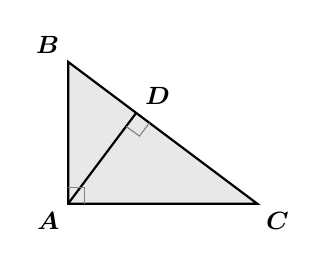
\begin{tikzpicture}[scale=0.6]

	\coordinate (A) at (0,0);
	\coordinate (B) at (0,3);
	\coordinate (C) at (4,0);
	% super cool tikzlibrary{calc} to get the point D on BC perpendicular from A
	\coordinate (D) at ($ (B)!(A)!(C) $);

	
  

	\small
	\filldraw[thick, fill=Gainsboro!65, draw=black] (A) -- (B) --  (C) --  cycle;
	\filldraw[thick, fill=Gainsboro!65, draw=black] (A) -- (D);
	\draw[gray, thin] ($ (D)+(-36.87:0.35) $) -- ++(233.13:0.35)-- +(144.13:0.35);
	\draw[gray, thin] (0,0.35) -- (0.35,0.35)-- (0.35,0);
  
	% \path (A) -- (C) node[midway, sloped, above] {$6.43\,$cm};
	% \path (C) -- (B) node[midway, sloped, above, rotate=180] {$5.26\,$cm};
	% \path (A) -- (B) node[midway, sloped, below] {$3.35\,$cm};
	\draw[below left] (A) node {$\bm A$};
	\draw[above left] (B) node {$\bm B$};
	\draw[below right] (C) node {$\bm C$};
	\draw[above right] (D) node {$\bm D$};

	% \draw ($ (A)+(54.7:1) $) arc (54.7:0:1)node[midway, fill=Gainsboro!65, inner sep=0.5mm,xshift=1mm] {\scriptsize $ 54.7\deg $};
  

	% \node[xshift=-0.5cm, yshift=0.15cm] at (C) {$\theta $};



\end{tikzpicture}
}
	}
\end{frame}


%%%%%%%%%%%%%%%%%%%%%%%%%%%%%%%%%%%%%%%%%%%%%%%%%%%%%%%%%%%%%%%%%%%%%%%%%%%%%%%%

\begin{frame}{Triangles and Trig Exercise}
	% \hspace{-.75cm}
	\mini[0.4]{
		\raggedright
		This is a standard type of statics problem to determine the forces in cables $AC$ and $BC$. But first we have to find the angles $\theta_{AC}$ and $\theta_{BC}$. This involves the use of the Pythagorean Theorem, the sine and cosine rules, and one of the trigonometric functions.
		\parb
		\begin{enumerate}
			\setcounter{enumi}{\themyexercisecounter}
			\item Find $\theta_{AC}$.
			\item Find $\theta_{BC}$.
			\setcounter{myexercisecounter}{\theenumi}
		\end{enumerate}
		% {\bfseries Don't give up yet!} Spend a few minutes and figure out how you can use the dimensions given to work towards finding angles $\theta_{AC}$ and $\theta_{BC}$.\parb
		% \textcolor{gray}{If you are really stuck, there are hints on the next slide :)}
	}
	\hfill
	\mini[0.55]{
		\begin{center}
			\tcb[left=2.5mm,right=2.5mm,top=3mm,bottom=3mm]{% !TEX root = ../../Beamer/statikz/statikz.tex


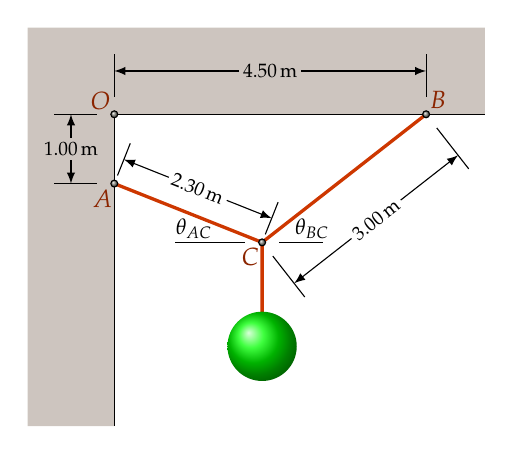
\begin{tikzpicture}[scale=0.88]

	\coordinate (O) at (0,0);
	\coordinate (B) at (4.5,0);
	\coordinate (BB) at ($(B)+(218:10)$);
	\coordinate (A) at (0,-1);
	\coordinate (AA) at ($(A)+(-21.7:10)$);
	% super cool tikzlibrary{calc} to get the intersection
	\coordinate (C) at (intersection of A--AA and B--BB);
	\coordinate (D) at ($ (C)+(0,-1.5) $);

	\fill[Seashell3] (O) -- ($ (B)+(0.85,0) $) --+(0,1.25)--(-1.25,1.25) -- (-1.25, -4.5) -- +(1.25,0)--cycle;
	\draw[thin] ($ (B)+(0.85,0) $) -- (O) -- ($ (A)+(0,-3.5) $);
	\draw[very thick, OrangeRed3] (A)--(C);
	\draw[very thick, OrangeRed3] (B)--(C);
	\draw[very thick, OrangeRed3] (C)--(D);
	\shade[ball color=green] (D) circle (.5cm);

	\draw[thin] ($ (C)+(0.25,0) $) --+(0.625,0);
	\draw[thin] ($ (C)+(-0.25,0) $) --+(-1,0);
	\node at ($ (C)+(15:0.75) $) {\footnotesize $ \theta_{BC} $};
	\node at ($ (C)+(169:1) $) {\footnotesize $ \theta_{AC} $};

	\draw[thin]  ($ (O)+(-0.25,0) $) --+(-0.625,0);
	\draw[thin]  ($ (A)+(-0.25,0) $) --+(-0.625,0);
	\draw[latex-latex] ($ (O)+(-0.625,0) $) -- node[fill=Seashell3, inner sep=0.5mm] {\scriptsize $1.00\,\text{m}$}($ (A)+(-0.625,0) $);

	
	\draw[thin]  ($ (O)+(0,0.25) $) --+(0, 0.625);
	\draw[thin]  ($ (B)+(0,0.25) $) --+(0, 0.625);
	\draw[latex-latex] ($ (O)+(0,.625) $) -- node[fill=Seashell3, inner sep=0.5mm] {\scriptsize $4.50\,\text{m}$}($ (B)+(0,0.625) $);

	
	
	\draw[thin]  ($ (C)+(-52:0.25) $) --+(-52:.75);
	\draw[thin]  ($ (B)+(-52:0.25) $) --+(-52:.75);
	\draw[latex-latex] ($(C)+(-52:0.75)$) -- node[fill=white, sloped, inner sep=0.5mm] {\scriptsize $3.00\,\text{m}$}($(B)+(-52:0.75)$);
	\draw[thin]  ($ (A)+(68.3:0.125) $) --+(68.3:0.5);
	\draw[thin]  ($ (C)+(68.3:0.125) $) --+(68.3:0.5);
	\draw[latex-latex] ($(A)+(68.3:0.375)$) -- node[fill=white, sloped, inner sep=0.5mm] {\scriptsize $2.30\,\text{m}$}($(C)+(68.3:0.375)$);

  
	\small
	\shadedraw [draw=black, ball color = Ivory4] (O) circle (0.05cm) node[OrangeRed4, xshift=-0.175cm, yshift=0.175cm] { $O$};
	\shadedraw [draw=black, ball color = Ivory4] (B) circle (0.05cm) node[OrangeRed4, xshift=0.15cm, yshift=0.1875cm] {$B$};
	\shadedraw [draw=black, ball color = Ivory4] (A) circle (0.05cm) node[OrangeRed4, xshift=-0.15cm, yshift=-0.1875cm] {$A$};
	\shadedraw [draw=black, ball color = Ivory4] (C) circle (0.05cm) node[OrangeRed4, xshift=-0.15cm, yshift=-0.1875cm] {$C$};



\end{tikzpicture}
}
		\end{center}
	}
	
\end{frame}





%%%%%%%%%%%%%%%%%%%%%%%%%%%%%%%%%%%%%%%%%%%%%%%%%%%%%%%%%%%%%%%%%%%%%%%%%%%%%%%

%%%%%%%%%%%%%%%%%%%%%%%%%%%%%%%%%%%%%%%%%%%%%%%%%%%%%%%%%%%%%%%%%%%%%%%%%%%%%%%

\begin{frame}{Simultaneous Equations}

	\mini[0.475]{
		\tcbox[colback=white,boxsep=0pt,top=5pt,bottom=5pt,left=5pt,
		right=5pt, colframe=structure]{
			\scalebox{.8}{
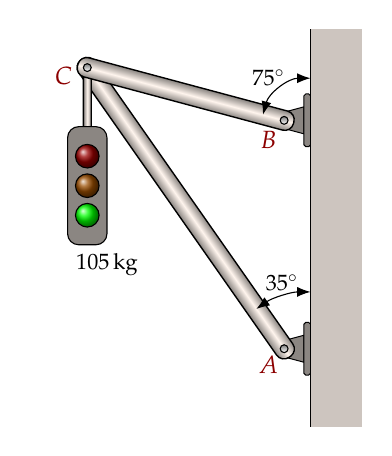
\begin{tikzpicture}[scale=0.5]

	\coordinate (C) at (0,0);
	\coordinate (B) at ($ (C)+(-15:5.176) $);
	\coordinate (A) at ($ (C)+(-55:8.717) $);
	\coordinate (D) at ($ (C)+(0,-3) $);

	\gettikzxy{(A)}{\ax}{\ay}
  \gettikzxy{(B)}{\bx}{\by}
  \gettikzxy{(C)}{\cx}{\cy}

	\PC[90]{B}{Seashell4}{black}{0.67}{0.125}
	\PC[90]{A}{Seashell4}{black}{0.67}{0.125}

	\fill[Seashell3] ($ (\bx+0.67cm, \cy+1cm) $) rectangle ($ (\ax+2cm, \ay-2cm) $);
	\draw[thin]  ($ (\bx+0.67cm, \cy+1cm) $) -- ($ (\bx+0.67cm, \ay-2cm) $);
	
	\Member{C}{A}{Seashell4}{Seashell1}{black}{0.5}{1.125}{0.5}	
	\Member{C}{D}{Seashell4}{Seashell1}{black}{0.2}{.125}{0.5}
	\Member{C}{B}{Seashell4}{Seashell1}{black}{0.5}{1.125}{0.5}

	\filldraw[rounded corners, fill=Seashell4] ($ (D)+(-0.5,-1.5) $) rectangle ($ (D)+(0.5,1.5) $);
	\shadedraw[ball color=orange!60!black] (D) circle (.3cm);
	\shadedraw[ball color=red!60!black] ($(D)+(0,0.75)$) circle (.3cm);
	\shadedraw[ball color=green] ($(D)+(0,-0.75)$) circle (.3cm);
	\node at ($ (D)-(-0.5,2) $) {\footnotesize $ 105\,$kg};

	\draw[Latex-Latex] ($ (B)+(-15:0.6936)+(0,1.25) $) arc (90:165:1.25) node[midway,xshift=-1.5mm, yshift=1.3mm] {\footnotesize $75\deg$};
	\draw[Latex-Latex] ($ (A)+(-55:1.168)+(0,2.4) $) arc (90:125:2.4) node[midway,yshift=1.75mm] {\footnotesize $35\deg$};

	\small
	
	\shadedraw [draw=black] (B) circle (0.1cm) node[statsMaroon, xshift=-0.2cm, yshift=-0.25cm] {$B$};
	\shadedraw [draw=black] (A) circle (0.1cm) node[statsMaroon, xshift=-0.2cm, yshift=-0.2cm] {$A$};
	\shadedraw [draw=black] (C) circle (0.1cm) node[statsMaroon, xshift=-0.3cm, yshift=-0.1cm] {$C$};

	\pgfresetboundingbox
	\draw[white] (\cx-1.5cm, \cy+1cm) rectangle (\ax+2cm, \ay-2cm);
	

\end{tikzpicture}


}
		}
	}
	\hfill
	\mini[0.475]{
		% \begin{flushright}
			\tcbox[colback=white,boxsep=0pt,top=5pt,bottom=5pt,left=5pt,
		right=5pt, colframe=structure]{
			\scalebox{.8}{% !TEX root = ../../Beamer/statikz/statikz.tex


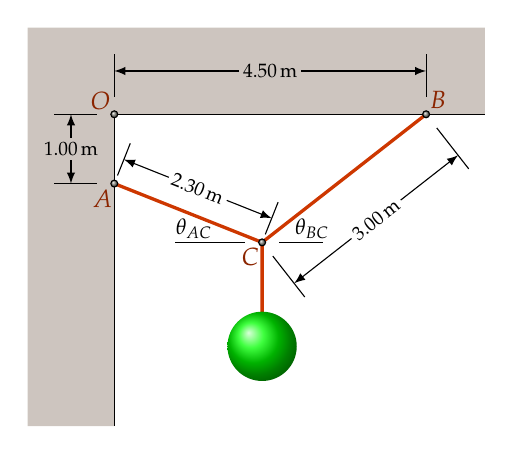
\begin{tikzpicture}[scale=0.88]

	\coordinate (O) at (0,0);
	\coordinate (B) at (4.5,0);
	\coordinate (BB) at ($(B)+(218:10)$);
	\coordinate (A) at (0,-1);
	\coordinate (AA) at ($(A)+(-21.7:10)$);
	% super cool tikzlibrary{calc} to get the intersection
	\coordinate (C) at (intersection of A--AA and B--BB);
	\coordinate (D) at ($ (C)+(0,-1.5) $);

	\fill[Seashell3] (O) -- ($ (B)+(0.85,0) $) --+(0,1.25)--(-1.25,1.25) -- (-1.25, -4.5) -- +(1.25,0)--cycle;
	\draw[thin] ($ (B)+(0.85,0) $) -- (O) -- ($ (A)+(0,-3.5) $);
	\draw[very thick, OrangeRed3] (A)--(C);
	\draw[very thick, OrangeRed3] (B)--(C);
	\draw[very thick, OrangeRed3] (C)--(D);
	\shade[ball color=green] (D) circle (.5cm);

	\draw[thin] ($ (C)+(0.25,0) $) --+(0.625,0);
	\draw[thin] ($ (C)+(-0.25,0) $) --+(-1,0);
	\node at ($ (C)+(15:0.75) $) {\footnotesize $ \theta_{BC} $};
	\node at ($ (C)+(169:1) $) {\footnotesize $ \theta_{AC} $};

	\draw[thin]  ($ (O)+(-0.25,0) $) --+(-0.625,0);
	\draw[thin]  ($ (A)+(-0.25,0) $) --+(-0.625,0);
	\draw[latex-latex] ($ (O)+(-0.625,0) $) -- node[fill=Seashell3, inner sep=0.5mm] {\scriptsize $1.00\,\text{m}$}($ (A)+(-0.625,0) $);

	
	\draw[thin]  ($ (O)+(0,0.25) $) --+(0, 0.625);
	\draw[thin]  ($ (B)+(0,0.25) $) --+(0, 0.625);
	\draw[latex-latex] ($ (O)+(0,.625) $) -- node[fill=Seashell3, inner sep=0.5mm] {\scriptsize $4.50\,\text{m}$}($ (B)+(0,0.625) $);

	
	
	\draw[thin]  ($ (C)+(-52:0.25) $) --+(-52:.75);
	\draw[thin]  ($ (B)+(-52:0.25) $) --+(-52:.75);
	\draw[latex-latex] ($(C)+(-52:0.75)$) -- node[fill=white, sloped, inner sep=0.5mm] {\scriptsize $3.00\,\text{m}$}($(B)+(-52:0.75)$);
	\draw[thin]  ($ (A)+(68.3:0.125) $) --+(68.3:0.5);
	\draw[thin]  ($ (C)+(68.3:0.125) $) --+(68.3:0.5);
	\draw[latex-latex] ($(A)+(68.3:0.375)$) -- node[fill=white, sloped, inner sep=0.5mm] {\scriptsize $2.30\,\text{m}$}($(C)+(68.3:0.375)$);

  
	\small
	\shadedraw [draw=black, ball color = Ivory4] (O) circle (0.05cm) node[OrangeRed4, xshift=-0.175cm, yshift=0.175cm] { $O$};
	\shadedraw [draw=black, ball color = Ivory4] (B) circle (0.05cm) node[OrangeRed4, xshift=0.15cm, yshift=0.1875cm] {$B$};
	\shadedraw [draw=black, ball color = Ivory4] (A) circle (0.05cm) node[OrangeRed4, xshift=-0.15cm, yshift=-0.1875cm] {$A$};
	\shadedraw [draw=black, ball color = Ivory4] (C) circle (0.05cm) node[OrangeRed4, xshift=-0.15cm, yshift=-0.1875cm] {$C$};



\end{tikzpicture}
}
		% \end{flushright}
		
	}
	}
	% centered minipage with text raggedright
	%cmini[width]{content}
	\cmini[0.8]{
		\centering
		Calculating the forces in $AC$ and $BC$ in each of the examples shown involves solving two equations in two unknowns \lb(also known as solving a system of simultaneous equations).\parm
		
		We'll review how to do this.
	}

\end{frame}
%%%%%%%%%%%%%%%%%%%%%%%%%%%%%%%%%%%%%%%%%%%%%%%%%%%%%%%%%%%%%%%%%%%%%%%%%%%%%%%%



\begin{frame}{Solving Simultaneous Equations}
	\cmini[0.8]{
		This is a simple system of simultaneous equations:
		\begin{align}
			2x + 3y & = 7 \\
			6x-y    & = 1
		\end{align}
		Our objective is to find the value of $x$ and $y$ that satisfies both equations.\pause
		\parb
		Equation (1) is a straight line, with slope $-2/3$, that intersects the $x$ axis at $x=3.5$ and intersects the $y$ axis at $y=7/3$. \parm
		Equation (2) is a straight line, with slope $6$, that intersects the $x$ axis at $x=1/6$ and intersects the $y$ axis at  $y=-1$. \parm
		\pause
		These lines have different slopes, so they must intersect somewhere. At the point $(x, \, y)$ where they intersect, both equations are satisfied. This is the solution we're looking for.
	}
\end{frame}
%%%%%%%%%%%%%%%%%%%%%%%%%%%%%%%%%%%%%%%%%%%%%%%%%%%%%%%%%%%%%%%%%%%%%%%%%%%%%%%%

\begin{frame}{Solving Simultaneous Equations (cont'd)}
	\mini[0.49]{
		\raggedright
		Graphically, the lines look like this. \parm
		It looks like the point at which they intersect is in the region of $(0.5,\, 2))$ \parm
		We can check whether this is the correct solution be substituting the values of $x=0.5$ and $y=2$ to see whether they satisfy both equations. \parm
		Generally, we can solve algebraically using a procedure called the Method of Subsitution. Or use the {\bf system-solver} on your calculator.\parm
		
		(The system-solver is allowed for quizzes and examinations; it saves time --- and improves accuracy when rushed. Make sure you know how your calculator works. Trying to figure it out in an exam is not recommended!)
	}
	\hfill
	\mini[0.47]{

		\begin{redbox}
			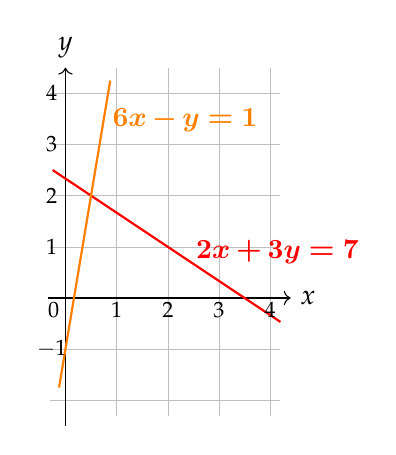
\begin{tikzpicture}[scale=0.65]
				\draw[very thin,color=gray!50] (-0.3,-2.3) grid (4.2,4.5);
				\draw[->] (-0.35,0) -- (4.4,0) node[right] {$x$};
				\draw[->] (0,-2.5) -- (0,4.5) node[above] {$y$};
    		\draw[color=red,domain=-0.25:4.2, thick] plot (\x,{-2/3*\x+7/3}) 
        	node[above right, xshift=-1.2cm, yshift=0.6cm,sloped] {$\bm{2x+3y=7}$};
    		\draw[color=orange,domain=-0.125:0.875, thick] plot (\x,{6*\x-1}) 
        	node[right,yshift=-0.5cm,xshift=-0.1cm] {$\bm{6x-y=1$}};
				\draw (0,0) node[xshift=-0.15cm, yshift=-0.15cm] {\footnotesize $0$};
				\draw (1,0) node[yshift=-0.15cm] {\footnotesize $1$};
				\draw (2,0) node[yshift=-0.15cm] {\footnotesize $2$};
				\draw (3,0) node[yshift=-0.15cm] {\footnotesize $3$};
				\draw (4,0) node[yshift=-0.15cm] {\footnotesize $4$};
				\draw (0,-1) node[xshift=-0.175cm] {\footnotesize $-1$};
				\draw (0,1) node[xshift=-0.175cm] {\footnotesize $1$};
				\draw (0,2) node[xshift=-0.175cm] {\footnotesize $2$};
				\draw (0,3) node[xshift=-0.175cm] {\footnotesize $3$};
				\draw (0,4) node[xshift=-0.175cm] {\footnotesize $4$};
			\end{tikzpicture}
			
		\end{redbox}
	}

\end{frame}

%%%%%%%%%%%%%%%%%%%%%%%%%%%%%%%%%%%%%%%%%%%%%%%%%%%%%%%%%%%%%%%%%%%%%%%%%%%%%%%%
% \begin{frame}
% 	\begin{tikzpicture}[scale=0.5]
% 		\begin{axis}[
% 			axis x line=middle, 
% 			axis y line=middle, 
% 			 ylabel=$y$, 
% 			xlabel=$x$
% 			]
%     	\addplot[domain=-10000:10000, blue, ultra thick, smooth] {14*x - x^2};
% 		\end{axis}
% 	\end{tikzpicture}
% 	\begin{tikzpicture}[scale=0.5]
% 		\begin{axis}[
% 			axis x line=middle, 
% 			axis y line=middle, 
% 			 ylabel=$y$, 
% 			xlabel=$x$
% 			]
%     	\addplot[domain=-0.125:0.875, blue, ultra thick, smooth] {6*\x-1};
%     	\addplot[domain=-0.25:3.7, orange, ultra thick, smooth] {-2/3*\x+7/3};
% 		\end{axis}
% 	\end{tikzpicture}
% \end{frame}

%%%%%%%%%%%%%%%%%%%%%%%%%%%%%%%%%%%%%%%%%%%%%%%%%%%%%%%%%%%%%%%%%%%%%%%%%%%%%%%%

\begin{frame}{Solving Simultaneous Equations using the Method of Subsitution}
	\small
	\cmini[0.8]{
		\setcounter{equation}{0}
		\begin{align}
			2x + 3y & = 7 \\
			6x-y    & = 1
		\end{align}
		The process:
		\begin{enumerate}[(a)]
			\item  Choose an equation and solve for one of the variables.
			      Here I choose equation (2) and solve for the variable $y$.
			      \begin{align}
			      	y & = 6x-1
			      \end{align}
			\item Use equation (3) to substitute $6x-1$ wherever $y$ occurs in the other equation:
			      \begin{align*}
			      	2x+3(6x-1) & = 7   \\
			      	2x+18x-3   & = 7   \\
			      	20x        & = 10  \\
			      	x          & = 0.5
			      \end{align*}
			\item Substitute this value for $x$ in either of equation (1) or (2):
			      \begin{align*}
			      	6x-y & = 1 \\
			      	3d-y & = 1 \\
			      	y    & = 2
			      \end{align*}
			\item We have our solution: $(0.5, \, 2)$.

		\end{enumerate}
	}
\end{frame}

%%%%%%%%%%%%%%%%%%%%%%%%%%%%%%%%%%%%%%%%%%%%%%%%%%%%%%%%%%%%%%%%%%%%%%%%%%%%%%%%

\begin{frame}{Typical Statics System of Equations}
	% left-aligned minipage with text raggedright
	%mini[width]{content}
	\mini[0.4]{
		\raggedright
		In an earlier exercise, we calculated that $\theta_{AC}=21.661\deg$ and
		$\theta_{BC}=38.049\deg$. \parm
		(Note that we are using 5 significant digits here because we will be using these values for calculations.)

	}
	\hfill
	\mini[0.53]{
		\vspace{0.375cm}
		\tcb[colback=white,boxsep=0pt,top=5pt,bottom=5pt,left=5pt,
		right=5pt, colframe=structure]{% !TEX root = ../../Beamer/statikz/statikz.tex


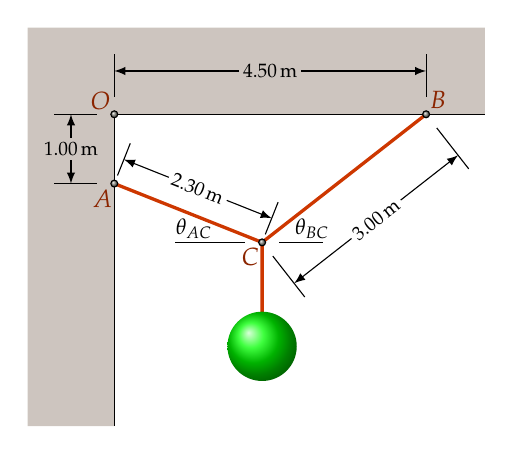
\begin{tikzpicture}[scale=0.88]

	\coordinate (O) at (0,0);
	\coordinate (B) at (4.5,0);
	\coordinate (BB) at ($(B)+(218:10)$);
	\coordinate (A) at (0,-1);
	\coordinate (AA) at ($(A)+(-21.7:10)$);
	% super cool tikzlibrary{calc} to get the intersection
	\coordinate (C) at (intersection of A--AA and B--BB);
	\coordinate (D) at ($ (C)+(0,-1.5) $);

	\fill[Seashell3] (O) -- ($ (B)+(0.85,0) $) --+(0,1.25)--(-1.25,1.25) -- (-1.25, -4.5) -- +(1.25,0)--cycle;
	\draw[thin] ($ (B)+(0.85,0) $) -- (O) -- ($ (A)+(0,-3.5) $);
	\draw[very thick, OrangeRed3] (A)--(C);
	\draw[very thick, OrangeRed3] (B)--(C);
	\draw[very thick, OrangeRed3] (C)--(D);
	\shade[ball color=green] (D) circle (.5cm);

	\draw[thin] ($ (C)+(0.25,0) $) --+(0.625,0);
	\draw[thin] ($ (C)+(-0.25,0) $) --+(-1,0);
	\node at ($ (C)+(15:0.75) $) {\footnotesize $ \theta_{BC} $};
	\node at ($ (C)+(169:1) $) {\footnotesize $ \theta_{AC} $};

	\draw[thin]  ($ (O)+(-0.25,0) $) --+(-0.625,0);
	\draw[thin]  ($ (A)+(-0.25,0) $) --+(-0.625,0);
	\draw[latex-latex] ($ (O)+(-0.625,0) $) -- node[fill=Seashell3, inner sep=0.5mm] {\scriptsize $1.00\,\text{m}$}($ (A)+(-0.625,0) $);

	
	\draw[thin]  ($ (O)+(0,0.25) $) --+(0, 0.625);
	\draw[thin]  ($ (B)+(0,0.25) $) --+(0, 0.625);
	\draw[latex-latex] ($ (O)+(0,.625) $) -- node[fill=Seashell3, inner sep=0.5mm] {\scriptsize $4.50\,\text{m}$}($ (B)+(0,0.625) $);

	
	
	\draw[thin]  ($ (C)+(-52:0.25) $) --+(-52:.75);
	\draw[thin]  ($ (B)+(-52:0.25) $) --+(-52:.75);
	\draw[latex-latex] ($(C)+(-52:0.75)$) -- node[fill=white, sloped, inner sep=0.5mm] {\scriptsize $3.00\,\text{m}$}($(B)+(-52:0.75)$);
	\draw[thin]  ($ (A)+(68.3:0.125) $) --+(68.3:0.5);
	\draw[thin]  ($ (C)+(68.3:0.125) $) --+(68.3:0.5);
	\draw[latex-latex] ($(A)+(68.3:0.375)$) -- node[fill=white, sloped, inner sep=0.5mm] {\scriptsize $2.30\,\text{m}$}($(C)+(68.3:0.375)$);

  
	\small
	\shadedraw [draw=black, ball color = Ivory4] (O) circle (0.05cm) node[OrangeRed4, xshift=-0.175cm, yshift=0.175cm] { $O$};
	\shadedraw [draw=black, ball color = Ivory4] (B) circle (0.05cm) node[OrangeRed4, xshift=0.15cm, yshift=0.1875cm] {$B$};
	\shadedraw [draw=black, ball color = Ivory4] (A) circle (0.05cm) node[OrangeRed4, xshift=-0.15cm, yshift=-0.1875cm] {$A$};
	\shadedraw [draw=black, ball color = Ivory4] (C) circle (0.05cm) node[OrangeRed4, xshift=-0.15cm, yshift=-0.1875cm] {$C$};



\end{tikzpicture}
}
	}
	\vspace{0.35cm}
	\cmini[0.8]{

		The system shown yields the following two equations:
		\begin{align*}
			% \setcounter{equation}{0}
			F_{AC}\sin\left(21.661^\circ\right) + F_{BC}\sin\left(38.049^\circ\right) & = 2011.1\,\text{N} \\
			F_{BC}\cos\left(38.049^\circ\right)-F_{AC}\cos\left(21.661^\circ\right)   & = 0
		\end{align*}

	}

\end{frame}
%%%%%%%%%%%%%%%%%%%%%%%%%%%%%%%%%%%%%%%%%%%%%%%%%%%%%%%%%%%%%%%%%%%%%%%%%%%%%%%%

\begin{frame}{System of Equations Exercise (1)}
	\cmini[0.8]{
		This looks more difficult than our previous example.
		\begin{align}
			\setcounter{equation}{0}
			F_{AC}\sin\left(21.661^\circ\right) + F_{BC}\sin\left(38.049^\circ\right) & = 2011.1 \\
			F_{BC}\cos\left(38.049^\circ\right)-F_{AC}\cos\left(21.661^\circ\right)   & = 0
		\end{align}
		Fortunately, it only {\bfseries looks} harder. $F_{AC}$ and $F_{BC}$ are variables, just like $x$ and $y$ in the earlier example.
		And the sines and cosines are just numbers. We get:
		\vspace{-0.125cm}
		\begin{align}
			0.36911x + 0.61633y & = 2011.1 \\
			0.78748y - 0.92938x & = 0
		\end{align}

		This is the same system, with $x$ replacing $F_{AC}$, $y$ replacing $F_{BC}$ and the trigonemetric functions evaluated.
		\parb
		\begin{enumerate}
			\setcounter{enumi}{\themyexercisecounter}
			\item Solve for $x$ ($F_{AC}$ in the original system) 
			% {\footnotesize\textcolor{gray}{\rotatebox[origin=c, y=2.5pt]{180}{(1830)}}}\\
			\item Solve for $y$ ($F_{BC}$ in the original system) 
			% {\footnotesize\textcolor{gray}{\rotatebox[origin=c, y=2.5pt]{180}{(2160)}}}
			      \setcounter{myexercisecounter}{\theenumi}
		\end{enumerate}
	}
\end{frame}

%%%%%%%%%%%%%%%%%%%%%%%%%%%%%%%%%%%%%%%%%%%%%%%%%%%%%%%%%%%%%%%%%%%%%%%%%%%%%%%%

\begin{frame}{System of Equations Exercise (2)}
	\mini[0.45]{
		\tcbox[colback=white,boxsep=0pt,top=5pt,bottom=5pt,left=5pt,
		right=5pt, colframe=structure]{
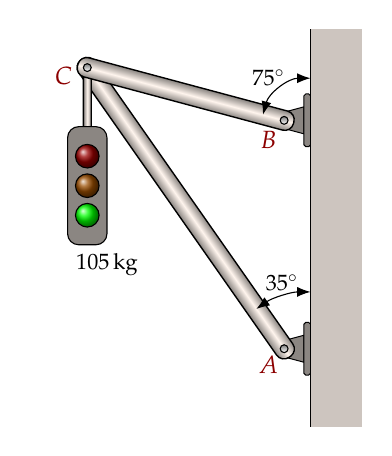
\begin{tikzpicture}[scale=0.5]

	\coordinate (C) at (0,0);
	\coordinate (B) at ($ (C)+(-15:5.176) $);
	\coordinate (A) at ($ (C)+(-55:8.717) $);
	\coordinate (D) at ($ (C)+(0,-3) $);

	\gettikzxy{(A)}{\ax}{\ay}
  \gettikzxy{(B)}{\bx}{\by}
  \gettikzxy{(C)}{\cx}{\cy}

	\PC[90]{B}{Seashell4}{black}{0.67}{0.125}
	\PC[90]{A}{Seashell4}{black}{0.67}{0.125}

	\fill[Seashell3] ($ (\bx+0.67cm, \cy+1cm) $) rectangle ($ (\ax+2cm, \ay-2cm) $);
	\draw[thin]  ($ (\bx+0.67cm, \cy+1cm) $) -- ($ (\bx+0.67cm, \ay-2cm) $);
	
	\Member{C}{A}{Seashell4}{Seashell1}{black}{0.5}{1.125}{0.5}	
	\Member{C}{D}{Seashell4}{Seashell1}{black}{0.2}{.125}{0.5}
	\Member{C}{B}{Seashell4}{Seashell1}{black}{0.5}{1.125}{0.5}

	\filldraw[rounded corners, fill=Seashell4] ($ (D)+(-0.5,-1.5) $) rectangle ($ (D)+(0.5,1.5) $);
	\shadedraw[ball color=orange!60!black] (D) circle (.3cm);
	\shadedraw[ball color=red!60!black] ($(D)+(0,0.75)$) circle (.3cm);
	\shadedraw[ball color=green] ($(D)+(0,-0.75)$) circle (.3cm);
	\node at ($ (D)-(-0.5,2) $) {\footnotesize $ 105\,$kg};

	\draw[Latex-Latex] ($ (B)+(-15:0.6936)+(0,1.25) $) arc (90:165:1.25) node[midway,xshift=-1.5mm, yshift=1.3mm] {\footnotesize $75\deg$};
	\draw[Latex-Latex] ($ (A)+(-55:1.168)+(0,2.4) $) arc (90:125:2.4) node[midway,yshift=1.75mm] {\footnotesize $35\deg$};

	\small
	
	\shadedraw [draw=black] (B) circle (0.1cm) node[statsMaroon, xshift=-0.2cm, yshift=-0.25cm] {$B$};
	\shadedraw [draw=black] (A) circle (0.1cm) node[statsMaroon, xshift=-0.2cm, yshift=-0.2cm] {$A$};
	\shadedraw [draw=black] (C) circle (0.1cm) node[statsMaroon, xshift=-0.3cm, yshift=-0.1cm] {$C$};

	\pgfresetboundingbox
	\draw[white] (\cx-1.5cm, \cy+1cm) rectangle (\ax+2cm, \ay-2cm);
	

\end{tikzpicture}


}
	}
	\hfill
	% centered minipage with text raggedright
	%cmini[width]{content}
	\mini[0.5]{
		The system shown yields the following two equations in the two unknowns $F_{AC}$ and $F_{BC}$:
		\begin{align*}
			F_{BC}\sin15^\circ + F_{AC}\cos35^\circ + 1030.1 & = 0 \\
			F_{BC}\cos 15^\circ+F_{AC}\sin35^\circ           & = 0
		\end{align*}
		\parb
		\begin{enumerate}
			\setcounter{enumi}{\themyexercisecounter}
			\item Determine $F_{AC}$
			%  {\footnotesize\textcolor{gray}{\rotatebox[origin=c, y=2.5pt]{180}{(-1550)}}}\\
			\item Determine $F_{BC}$
			%  {\footnotesize\textcolor{gray}{\rotatebox[origin=c, y=2.5pt]{180}{(919)}}}
			      \setcounter{myexercisecounter}{\theenumi}
		\end{enumerate}
	}



\end{frame}
%%%%%%%%%%%%%%%%%%%%%%%%%%%%%%%%%%%%%%%%%%%%%%%%%%%%%%%%%%%%%%%%%%%%%%%%%%%%%%%%
%%%%%%%%%%%%%%%%%%%%%%%%%%%%%%%%%%%%%%%%%%%%%%%%%%%%%%%%%%%%%%%%%%%%%%%%%%%%%%%%
%%%%%%%%%%%%%%%%%%%%%%%%%%%%%%%%%%%%%%%%%%%%%%%%%%%%%%%%%%%%%%%%%%%%%%%%%%%%%%%%
%%%%%%%%%%%%%%%%%%%%%%%%%%%%%%%%%%%%%%%%%%%%%%%%%%%%%%%%%%%%%%%%%%%%%%%%%%%%%%%%
%%%%%%%%%%%%%%%%%%%%%%%%%%%%%%%%%%%%%%%%%%%%%%%%%%%%%%%%%%%%%%%%%%%%%%%%%%%%%%%%
%%%%%%%%%%%%%%%%%%%%%%%%%%%%%%%%%%%%%%%%%%%%%%%%%%%%%%%%%%%%%%%%%%%%%%%%%%%%%%%%
%%%%%%%%%%%%%%%%%%%%%%%%%%%%%%%%%%%%%%%%%%%%%%%%%%%%%%%%%%%%%%%%%%%%%%%%%%%%%%%%
%%%%%%%%%%%%%%%%%%%%%%%%%%%%%%%%%%%%%%%%%%%%%%%%%%%%%%%%%%%%%%%%%%%%%%%%%%%%%%%%
%%%%%%%%%%%%%%%%%%%%%%%%%%%%%%%%%%%%%%%%%%%%%%%%%%%%%%%%%%%%%%%%%%%%%%%%%%%%%%%%
%%%%%%%%%%%%%%%%%%%%%%%%%%%%%%%%%%%%%%%%%%%%%%%%%%%%%%%%%%%%%%%%%%%%%%%%%%%%%%%%
%%%%%%%%%%%%%%%%%%%%%%%%%%%%%%%%%%%%%%%%%%%%%%%%%%%%%%%%%%%%%%%%%%%%%%%%%%%%%%%%
%%%%%%%%%%%%%%%%%%%%%%%%%%%%%%%%%%%%%%%%%%%%%%%%%%%%%%%%%%%%%%%%%%%%%%%%%%%%%%%%
%%%%%%%%%%%%%%%%%%%%%%%%%%%%%%%%%%%%%%%%%%%%%%%%%%%%%%%%%%%%%%%%%%%%%%%%%%%%%%%%
%%%%%%%%%%%%%%%%%%%%%%%%%%%%%%%%%%%%%%%%%%%%%%%%%%%%%%%%%%%%%%%%%%%%%%%%%%%%%%%%
%%%%%%%%%%%%%%%%%%%%%%%%%%%%%%%%%%%%%%%%%%%%%%%%%%%%%%%%%%%%%%%%%%%%%%%%%%%%%%%%
%%%%%%%%%%%%%%%%%%%%%%%%%%%%%%%%%%%%%%%%%%%%%%%%%%%%%%%%%%%%%%%%%%%%%%%%%%%%%%%%
%%%%%%%%%%%%%%%%%%%%%%%%%%%%%%%%%%%%%%%%%%%%%%%%%%%%%%%%%%%%%%%%%%%%%%%%%%%%%%%%
%%%%%%%%%%%%%%%%%%%%%%%%%%%%%%%%%%%%%%%%%%%%%%%%%%%%%%%%%%%%%%%%%%%%%%%%%%%%%%%%
%%%%%%%%%%%%%%%%%%%%%%%%%%%%%%%%%%%%%%%%%%%%%%%%%%%%%%%%%%%%%%%%%%%%%%%%%%%%%%%%
%%%%%%%%%%%%%%%%%%%%%%%%%%%%%%%%%%%%%%%%%%%%%%%%%%%%%%%%%%%%%%%%%%%%%%%%%%%%%%%%
%%%%%%%%%%%%%%%%%%%%%%%%%%%%%%%%%%%%%%%%%%%%%%%%%%%%%%%%%%%%%%%%%%%%%%%%%%%%%%%%
%%%%%%%%%%%%%%%%%%%%%%%%%%%%%%%%%%%%%%%%%%%%%%%%%%%%%%%%%%%%%%%%%%%%%%%%%%%%%%%%
%%%%%%%%%%%%%%%%%%%%%%%%%%%%%%%%%%%%%%%%%%%%%%%%%%%%%%%%%%%%%%%%%%%%%%%%%%%%%%%%
%%%%%%%%%%%%%%%%%%%%%%%%%%%%%%%%%%%%%%%%%%%%%%%%%%%%%%%%%%%%%%%%%%%%%%%%%%%%%%%%
%%%%%%%%%%%%%%%%%%%%%%%%%%%%%%%%%%%%%%%%%%%%%%%%%%%%%%%%%%%%%%%%%%%%%%%%%%%%%%%%
%%%%%%%%%%%%%%%%%%%%%%%%%%%%%%%%%%%%%%%%%%%%%%%%%%%%%%%%%%%%%%%%%%%%%%%%%%%%%%%%
%%%%%%%%%%%%%%%%%%%%%%%%%%%%%%%%%%%%%%%%%%%%%%%%%%%%%%%%%%%%%%%%%%%%%%%%%%%%%%%%
%%%%%%%%%%%%%%%%%%%%%%%%%%%%%%%%%%%%%%%%%%%%%%%%%%%%%%%%%%%%%%%%%%%%%%%%%%%%%%%%
%%%%%%%%%%%%%%%%%%%%%%%%%%%%%%%%%%%%%%%%%%%%%%%%%%%%%%%%%%%%%%%%%%%%%%%%%%%%%%%%
%%%%%%%%%%%%%%%%%%%%%%%%%%%%%%%%%%%%%%%%%%%%%%%%%%%%%%%%%%%%%%%%%%%%%%%%%%%%%%%%
%%%%%%%%%%%%%%%%%%%%%%%%%%%%%%%%%%%%%%%%%%%%%%%%%%%%%%%%%%%%%%%%%%%%%%%%%%%%%%%%
%%%%%%%%%%%%%%%%%%%%%%%%%%%%%%%%%%%%%%%%%%%%%%%%%%%%%%%%%%%%%%%%%%%%%%%%%%%%%%%%
%%%%%%%%%%%%%%%%%%%%%%%%%%%%%%%%%%%%%%%%%%%%%%%%%%%%%%%%%%%%%%%%%%%%%%%%%%%%%%%%
%%%%%%%%%%%%%%%%%%%%%%%%%%%%%%%%%%%%%%%%%%%%%%%%%%%%%%%%%%%%%%%%%%%%%%%%%%%%%%%%
%%%%%%%%%%%%%%%%%%%%%%%%%%%%%%%%%%%%%%%%%%%%%%%%%%%%%%%%%%%%%%%%%%%%%%%%%%%%%%%%

\end{document}

%%%%%%%%%%%%%%%%%%%%%%%%%%%%%%%%%%%%%%%%%%%%%%%%%%%%%%%%%%%%%%%%%%%%%%%%%%%%%%%%